%Nguyễn Cường
\Opensolutionfile{ans}
\section{KHÁI NIỆM VỀ MẶT TRÒN XOAY}
\subsection{KIẾN THỨC SÁCH GIÁO KHOA CẦN NẮM}
\subsubsection{SỰ TẠO THÀNH MẶT TRÒN XOAY}
\immini{
– Trong không gian cho mặt phẳng $(P)$ chứa đường thẳng $\Delta$ và một đường $\mathscr{C}$. Khi quay mặt phẳng $(P)$ quanh $\Delta$ một góc $360^{\circ}$ thì mỗi điểm $M$ trên $\mathscr{C}$ vạch ra một đường tròn có tâm $O$ thuộc $\Delta$ và nằm trên mặt phẳng vuông góc với $\Delta$. Như vậy khi quay mặt phẳng $(P)$ quanh đường thẳng $\Delta$ thì $\mathscr{C}$ sẽ tạo nên được một hình gọi là mặt tròn xoay.\\
– Trong đó: đường $\mathscr{C}$ được gọi là đường sinh của mặt nón; đường thẳng $\Delta$ được gọi là trục của mặt tròn xoay. 
}
{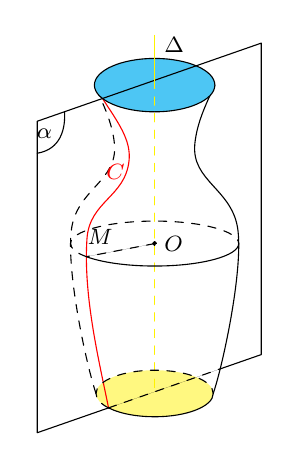
\begin{tikzpicture}[scale=.7,line join=round, line cap = round,font=\footnotesize]
	\fill[yellow!50](1.0635,0.765)
	.. controls (1.0635,0.532) and (0.58725,0.343) .. (0,0.343)
	.. controls (-0.267,0.34275) and (-0.59425,0.38325) .. (-0.836,0.504)
	.. controls (-0.97875,0.57575) and (-1.06375,0.6665) .. (-1.06375,0.765)
	.. controls (-1.06375,0.99825) and (-0.5875,1.187) .. (0,1.187)
	.. controls (0.58725,1.187) and (1.0635,0.99825) .. (1.0635,0.765);
	\draw[dashed] (-1.0635,0.76525)
	.. controls (-1.24,1.28575) and (-1.59975,2.955) .. (-1.5125,3.71825)
	.. controls (-1.42625,4.4745) and (-0.66225,4.606) .. (-0.7295,5.29425)
	.. controls (-0.76625,5.67) and (-0.928,6.0105) .. (-1.093,6.35975);
	\draw[red] (-0.836,0.504)
	.. controls (-1.0135,1.37725) and (-1.295,2.5325) .. (-1.22825,3.56575)
	.. controls (-1.1835,4.25775) and (-0.53725,4.32275) .. (-0.4645,4.9865)node[shift={(-.1,.1)},pos=.8]{$\mathscr{C}$}
	.. controls (-0.42275,5.36575) and (-0.6695,5.691) .. (-0.946,6.117);
	\draw (1.0635,0.765)
	.. controls (1.2395,1.28575) and (1.59925,2.95475) .. (1.51225,3.71825)
	.. controls (1.426,4.474) and (0.66175,4.606) .. (0.72925,5.29425)
	.. controls (0.76625,5.67) and (0.92775,6.0105) .. (1.0925,6.35975);
	\draw[fill=cyan!70] (0,6.84375)
	.. controls (0.60325,6.84375) and (1.0925,6.627) .. (1.0925,6.35975)
	.. controls (1.0925,6.09225) and (0.60325,5.8755) .. (0,5.8755)
	.. controls (-0.60375,5.8755) and (-1.093,6.09225) .. (-1.093,6.35975)
	.. controls (-1.093,6.627) and (-0.60375,6.84375) .. cycle;
	\draw (-0.836,0.504)--(-2.13,.053)--(-2.13,5.704)--(1.935,7.122)--(1.935,1.471)--(1.189,1.211);
	\draw[yellow] (0,6.447)--(0,7.26)node[right,pos=.8,black]{$\Delta$};
	\draw[thin,dashed,yellow] (0,6.447)--(0,0.796);
	\draw[thin,dashed] (-0.836,0.504)--(1.189,1.211) [fill=black](0,3.485) circle (1pt)--(-1.238,3.247)node[right,pos=0]{$O$}node[above,pos=.8]{$M$};
	\draw (-2.1295,5.12475)
	.. controls (-1.8015,5.17475) and (-1.60975,5.433) .. (-1.6345,5.877)node[left,pos=.65]{$\alpha$};
	\draw (1.52525,3.48525)
	.. controls (1.52525,3.26) and (0.84225,3.07725) .. (0,3.07725)
	.. controls (-0.51,3.07725) and (-0.96125,3.14425) .. (-1.23825,3.24675);
	\draw[dashed] (-1.23825,3.24675)
	.. controls (-1.419,3.31375) and (-1.5255,3.39625) .. (-1.5255,3.485)
	.. controls (-1.5255,3.71025) and (-0.8425,3.893) .. (0,3.893)
	.. controls (0.84225,3.893) and (1.52525,3.71025) .. (1.52525,3.485);
	\draw (1.0635,0.765)
	.. controls (1.0635,0.532) and (0.58725,0.343) .. (0,0.343)
	.. controls (-0.267,0.34275) and (-0.59425,0.38325) .. (-0.836,0.504);
	\draw[dashed] (-0.836,0.504)
	.. controls (-0.97875,0.57575) and (-1.06375,0.6665) .. (-1.06375,0.765)
	.. controls (-1.06375,0.99825) and (-0.5875,1.187) .. (0,1.187)
	.. controls (0.58725,1.187) and (1.0635,0.99825) .. (1.0635,0.765);
	\end{tikzpicture}
}
\subsubsection{MẶT NÓN TRÒN XOAY}
\textbf{1. Định nghĩa mặt nón tròn xoay.}
\immini{
– Trong mặt phẳng $(P)$ cho hai đường thẳng $d$ và $\Delta$ cắt nhau tại điểm $O$ và tạo thành góc $\alpha$ (với $0^{\circ}<\alpha<90^{\circ}$). Khi quay mặt phẳng $(P)$ xung quanh $\Delta$ thì đường thẳng $d$ sinh ra một mặt tròn xoay được gọi là mặt nón tròn xoay đỉnh $O$.\\
– Gọi tắt là mặt nón tròn xoay.\\
– Trong đó: Đường thẳng $\Delta$ được gọi là trục; đường thẳng $d$ được gọi là đường sinh; góc $2\alpha$ được gọi là góc ở đỉnh.}
{
	\tdplotsetmaincoords{72}{160}
	\begin{tikzpicture}[line join=round,line cap=round,tdplot_main_coords,very thin]
	\def\a{2} \def\h{4}
	\pgfmathsetmacro\b{\a*sqrt(2)}
	\draw (0,0,0) circle (\a);
	\path
	(\b,0,0) coordinate (A) (0,-\b,0) coordinate (B) (-\b,0,0)coordinate (C) (0,\b,0) coordinate (D)
	(\a,0,0) coordinate(M) (-\a,0,0) coordinate(N) (0,\a,0) coordinate(K) (0,-\a,0) coordinate(L)
	(barycentric cs:A=1,B=1)coordinate(P) (barycentric cs:C=1,D=1)coordinate(Q)
	(M)+(0,0,-\h) coordinate(M') (N)+(0,0,-\h) coordinate(N')
	(K)+(0,0,-\h) coordinate(K') (L)+(0,0,-\h) coordinate(L')
	(P)+(0,0,-\h) coordinate(P') (Q)+(0,0,-\h) coordinate(Q');
	\draw(M)--(N')node[right]{$d$} (P')--(Q)(K')--(0,0,-\h/2)node[right]{$O$}(L)--(0,0,0)--(0,0,\h/3)(0,0,-\h-\h/3)--(0,0,-\h-\h/6);
	\draw[dashed](L)--(0,0,-\h/2)(0,0,0)node[right]{$\Delta$}--(0,0,-\h)--(K')(0,0,-\h)--(0,0,-\h-\h/6);
	\draw[fill=white](0,0,-\h/2)circle(.5pt) (0,0,0)circle(.5pt) (0,0,-\h)circle(.5pt) (K')circle(.5pt) (L)circle(.5pt);
	\draw[densely dotted](N')arc(-180:-45:\a);
	\draw(N')arc(180:-45:\a);
	\end{tikzpicture}}
\noindent\textbf{2. Hình nón tròn xoay và khối nón tròn xoay.}
\immini{
\textbf{a) Hình nón tròn xoay.}\\
– Cho $\triangle IAB$ vuông tại $I$. Khi quay tam giác đó xung quanh cạnh góc vuông $AI$ thì đường gấp khúc $IBA$ tạo thành một hình được gọi là hình nón tròn xoay, gọi tắt là hình nón.\\
– Trong đó:
\begin{itemize}
	\item Hình tròn tâm $I$ sinh bởi các điểm thuộc cạnh $IB$ khi $IB$ quay quanh trục $AI$ được gọi là mặt đáy của mình nón.
	\item Điểm $O$ được gọi là đỉnh của hình nón.
	\item Độ dài đoạn $AI$ được gọi là chiều cao của hình nón.
	\item Độ dài đoạn $AB$ được gọi là độ dài đường sinh của hình nón.
	\item Phần mặt tròn xoay sinh bởi các điểm trên cạnh $AB$ khi quay quanh $AI$ được gọi là mặt xung quanh của hình nón.
\end{itemize}}
 {
 	\begin{tikzpicture}[scale=0.6, font=\footnotesize, line join = round, line cap = round, >=stealth]
 	\def\x{3}
 	\def\y{1}
 	\coordinate[label=right:B] (B) at (0,0);
 	\coordinate (D) at (-6,0);
 	\coordinate (r) at (-3,-1);
 	\coordinate[label=left:I] (I) at ($(D)!0.5!(B)$);
 	\coordinate[label=above:A] (A) at ($(I)+(0,6)$);	
 	\coordinate (l) at ($(A)!0.5!(B)$);
 	\draw[dashed] (B) arc (0:180:3 cm and 1cm);
 	\draw (B) arc (0:-180:3 cm and 1cm);
 	\draw (A)--(D)
 	(A)--(B)node[pos=0.5,left] {$l$};
 	\draw[dashed] (A)--(I)node[pos=0.5,left] {$h$}
 	(I)--(B)node[pos=0.5,below] {$r$};
 	%\pic[draw=black,<->,"$\alpha$", angle eccentricity=0.05cm,angle radius=0.5cm]{angle=I--A--B};
 	\end{tikzpicture}
 }
\immini{
\textbf{b) Khối nón tròn xoay.}\\
– Phần không gian được giới hạn bởi một hình nón tròn xoay kể cả hình đó được gọi là khối nón tròn xoay hay còn gọi tắt là khối nón.\\
– Trong đó
\begin{itemize}
	\item Điểm thuộc khối nón nhưng không thuộc hình nón gọi là điểm trong của khối nón.
	\item Ta gọi đỉnh, mặt đáy, đường sinh của hình nón theo thứ tự là đỉnh, mặt đáy, đường sinh của khối nón tương ứng.
\end{itemize}
}
{\begin{tikzpicture}[scale=.7,line join=round]
	\def\a{4} % bán trục lớn của ellip đáy
	\def\b{1.5} % bán trục nhỏ của ellip đáy
	\def\h{4} % chiều cao nón
	\coordinate (S) at (0,\h);
	\coordinate (A) at (\a,0);
	\coordinate (B) at (-\a,0);
	\coordinate (C) at (0,\b);
	\coordinate (D) at (0,-\b);
	\coordinate (O) at (0,0);
	% xác định các giao điểm I,J của 2 cạnh bên và ellip đáy
	\path[name path=2sides] (A)--(S)--(B);
	\path[name path=baseellipse] (0,0) ellipse [x radius=\a, y radius=\b];
	\path[name intersections={of=baseellipse and 2sides}]
	(intersection-2) coordinate (I)
	(intersection-3) coordinate (J);
	\coordinate (E) at (intersection of A--D and C--I);
	\coordinate (F) at (intersection of A--C and D--I);
	\path[name path=EF] (E)--(F);
	\path[name intersections={of=baseellipse and EF,by={H}}];
	\coordinate (K) at (intersection of B--D and C--J);
	\coordinate (L) at (intersection of B--C and D--J);
	\path[name path=KL] (K)--(L);
	\path[name intersections={of=baseellipse and KL,by={G}}];
	% Tính góc tham số tH của H, tG của G
	\newdimen\xH
	\newdimen\yH
	\path (H); % cho đầu bút vẽ về (H)
	\pgfgetlastxy{\xH}{\yH};
	\pgfmathsetmacro{\tH}{atan2(\a*\yH,\b*\xH)};
	\newdimen\xG
	\newdimen\yG
	\path (G); % cho đầu bút vẽ về (G)
	\pgfgetlastxy{\xG}{\yG};
	\pgfmathsetmacro{\tG}{atan2(\a*\yG,\b*\xG)};
	\pgfresetboundingbox
	% Vẽ các cung elip
	\filldraw[draw=cyan,top color=cyan!10, bottom color=cyan] (S)--(G) arc[start angle=\tG,end angle=360+\tH,x radius=\a,y radius=\b]--cycle;
	\draw[cyan,dashed,opacity=.5] (H) arc[start angle=\tH, end angle= \tG,x radius=\a, y radius=\b];
	\draw[magenta!50,dashed] (O)--(S) (O)--(A) (O)--(B);
	\draw[cyan] (S)--(A) (S)--(B);
	\end{tikzpicture}}
\noindent\textbf{3. Diện tích xung quanh và diện tích toàn phần của khối nón tròn xoay.}
\immini{\textbf{a) Diện tích xung quanh của hình nón.}\\
– Diện tích xung quanh của hình nón tròn xoay là giới hạn của diện tích xung quanh của hình chóp đều nội tiếp hình nón đó khi số cạnh tăng lên vô hạn.\\
– Công thức $S_{\text{xq}}=\pi rl$.\\
Trong đó $r$ là bán kính đáy; $l$ là độ dài đường sinh.}{\begin{tikzpicture}[scale=.7,line join=round]
\def\a{4} % bán trục lớn của ellip đáy
\def\b{1.5} % bán trục nhỏ của ellip đáy
\def\h{4} % chiều cao nón
\coordinate (S) at (0,\h);
\coordinate (A) at (\a,0);
\coordinate (B) at (-\a,0);
\coordinate (C) at (0,\b);
\coordinate (D) at (0,-\b);
\coordinate (O) at (0,0);
% xác định các giao điểm I,J của 2 cạnh bên và ellip đáy
\path[name path=2sides] (A)--(S)--(B);
\path[name path=baseellipse] (0,0) ellipse [x radius=\a, y radius=\b];
\path[name intersections={of=baseellipse and 2sides}]
(intersection-2) coordinate (I)
(intersection-3) coordinate (J);
\coordinate (E) at (intersection of A--D and C--I);
\coordinate (F) at (intersection of A--C and D--I);
\path[name path=EF] (E)--(F);
\path[name intersections={of=baseellipse and EF,by={H}}];
\coordinate (K) at (intersection of B--D and C--J);
\coordinate (L) at (intersection of B--C and D--J);
\path[name path=KL] (K)--(L);
\path[name intersections={of=baseellipse and KL,by={G}}];
% Tính góc tham số tH của H, tG của G
\newdimen\xH
\newdimen\yH
\path (H); % cho đầu bút vẽ về (H)
\pgfgetlastxy{\xH}{\yH};
\pgfmathsetmacro{\tH}{atan2(\a*\yH,\b*\xH)};
\newdimen\xG
\newdimen\yG
\path (G); % cho đầu bút vẽ về (G)
\pgfgetlastxy{\xG}{\yG};
\pgfmathsetmacro{\tG}{atan2(\a*\yG,\b*\xG)};
\pgfresetboundingbox
% Vẽ các cung elip
\filldraw[draw=cyan,top color=cyan!10, bottom color=cyan] (S)--(G) arc[start angle=\tG,end angle=360+\tH,x radius=\a,y radius=\b]--cycle;
\draw[cyan,dashed,opacity=.5] (H) arc[start angle=\tH, end angle= \tG,x radius=\a, y radius=\b];
\draw[magenta!50,dashed] (O)--(S) (O)--(A) (O)--(B);
\draw[cyan] (S)--(A) (S)--(B);
\end{tikzpicture}}
\immini{\textbf{b) Diện tích toàn phần của hình nón.}\\
– Diện tích toàn phần của hình nón tròn xoay là tổng diện tích mặt đáy với diện tích xung quanh của hình nón tròn xoay.\\
– Công thức $S_{\text{tp}}=\pi rl+\pi r^2$.} {\begin{tikzpicture}[scale=.7,line join=round]
	\def\a{4} % bán trục lớn của ellip đáy
	\def\b{1.5} % bán trục nhỏ của ellip đáy
	\def\h{4} % chiều cao nón
	\coordinate (S) at (0,\h);
	\coordinate (A) at (\a,0);
	\coordinate (B) at (-\a,0);
	\coordinate (C) at (0,\b);
	\coordinate (D) at (0,-\b);
	\coordinate (O) at (0,0);
	% xác định các giao điểm I,J của 2 cạnh bên và ellip đáy
	\path[name path=2sides] (A)--(S)--(B);
	\path[name path=baseellipse] (0,0) ellipse [x radius=\a, y radius=\b];
	\path[name intersections={of=baseellipse and 2sides}]
	(intersection-2) coordinate (I)
	(intersection-3) coordinate (J);
	\coordinate (E) at (intersection of A--D and C--I);
	\coordinate (F) at (intersection of A--C and D--I);
	\path[name path=EF] (E)--(F);
	\path[name intersections={of=baseellipse and EF,by={H}}];
	\coordinate (K) at (intersection of B--D and C--J);
	\coordinate (L) at (intersection of B--C and D--J);
	\path[name path=KL] (K)--(L);
	\path[name intersections={of=baseellipse and KL,by={G}}];
	% Tính góc tham số tH của H, tG của G
	\newdimen\xH
	\newdimen\yH
	\path (H); % cho đầu bút vẽ về (H)
	\pgfgetlastxy{\xH}{\yH};
	\pgfmathsetmacro{\tH}{atan2(\a*\yH,\b*\xH)};
	\newdimen\xG
	\newdimen\yG
	\path (G); % cho đầu bút vẽ về (G)
	\pgfgetlastxy{\xG}{\yG};
	\pgfmathsetmacro{\tG}{atan2(\a*\yG,\b*\xG)};
	\pgfresetboundingbox
	% Vẽ các cung elip
	\filldraw[draw=cyan,top color=cyan!10, bottom color=cyan] (S)--(G) arc[start angle=\tG,end angle=360+\tH,x radius=\a,y radius=\b]--cycle;
	\draw[cyan,dashed,opacity=.5] (H) arc[start angle=\tH, end angle= \tG,x radius=\a, y radius=\b];
	\draw[magenta!50,dashed] (O)--(S) (O)--(A) (O)--(B);
	\draw[cyan] (S)--(A) (S)--(B);
	\end{tikzpicture}}
\immini{
\textbf{c) Diện tích hình quạt.}\\
– Nếu cắt mặt xung quanh của hình nón theo một đường sinh rồi trải ra trên một mặt phẳng thì ta sẽ được:\\
+ Một hình quạt có bán hính bằng độ dài đường sinh của hình nón.\\
+ Một cung tròn có độ dài bằng chu vi đường tròn đáy của hình nón.\\
– Công thức: $S_{\text{xq}}=S_{\text{quạt}}=\pi rl$}{\begin{tikzpicture}[scale=0.6, font=\footnotesize, line join = round, line cap = round, >=stealth]
\draw(-4,0)--(0,0) arc (0:-150:4)node[above left]{$2\pi r$}--cycle;
\draw (1.5,0)circle(1.5);
\draw (0,0)--(1.5,0)node[midway,above]{$r$};
\draw (-2,0)node[above]{$l$};
;
\end{tikzpicture}}
\noindent\textbf{4. Thể tích của khối nón tròn xoay.}\\
\immini{– Thể tích của khối nón tròn xoay là giới hạn của thể tích khối chóp đều nội tiếp khối nón khi đó số cạnh tăng lên vô hạn.\\
– Công thức:$V=\dfrac{1}{3} \cdot S_{\text{đáy}}\cdot h$. Trong đó: $h$ là chiều cao của khối nón.\\
– Nếu đáy là hình tròn có bán kính $r$ thì $V=\dfrac{1}{3}\pi r^2h$.} 
{\begin{tikzpicture}[scale=.5,line cap=round,line join=round]
	\def \x{3}
	\def \y{1.5}
	\def \z{6}
	\def \an{108}% 70<\an<110 Góc quay của điểm A.
	\def \be{10}% 0<\be<10 
	\coordinate (I) at (0,0);
	\coordinate (O) at ($(I)+(0,\z)$);
	\coordinate (G) at ($(I) + (0+\be:{\x} and {\y})$);
	\coordinate (H) at ($(I) + (180-\be:{\x} and {\y})$);
	\coordinate (A) at ($(I) + (\an:{\x} and {\y})$);
	\coordinate (B) at ($(I) + (\an+60:{\x} and {\y})$);
	\coordinate (C) at ($(B)-(A)$);
	\coordinate (D) at ($(C)-(B)$);
	\coordinate (E) at ($(D)-(C)$);
	\coordinate (F) at ($(E)-(D)$);
	\draw [dashed] (A)--(B)--(C)--(D)--(E)--(F)--(A);
	\draw[dashed] (10:{\x} and {\y}) arc (10:170:{\x} and {\y});
	\draw (170:{\x} and {\y}) arc (170:370:{\x} and {\y});
	\draw[dashed] (O)--(A) (O)--(B) (O)--(D) (O)--(F) (O)--(I);
	\draw (O)--(C) (O)--(E) (O)--(G) (O)--(H);
	\end{tikzpicture}}
\noindent\textbf{5. Hình nón cụt.}\\
\immini{– Hình nón cụt là phần nón giới hạn bởi mặt đáy và một thiết diện song song với đáy.\\
– Công thức.\\
+ Diện tích xung quanh $S_{\text{xq}}=\pi(R+r)l$.\\
+ Diện tích toàn phần $S_{\text{tp}}=\pi(R+r)l +\pi(R^2+r^2)$.\\
+ Thể tích khối nón cụt $V=\dfrac{1}{3}\pi h\left(R^2+r^2+Rr\right)$.\\
Trong đó: $R, r$ là bán kính hai đáy; $h$ là độ cao hình chóp cụt.} 
{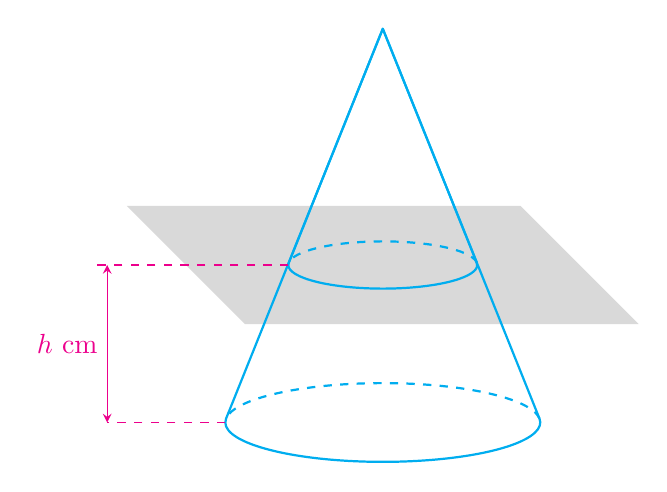
\begin{tikzpicture}[>=stealth,line join=round]
	\def\a{2} % major
	\def\b{.5} % minor
	\def\h{5} % height of the cone
	\def\d{3} % height of the section
	\pgfmathsetmacro{\t}{asin(\b/\h)}
	\fill[gray!30,shift={(90:\h-\d)},scale=2.5,xslant=-1,yscale=.3] (-1,1) rectangle (1,-1);
	\begin{scope}[cyan,thick]
	\draw[dashed]
	(\t:{\a} and {\b}) arc(\t:180-\t:{\a} and {\b});
	\draw
	(\t:{\a} and {\b})--(0,\h)--(180-\t:{\a} and {\b})
	arc(180-\t:360+\t:{\a} and {\b});
	\begin{scope}[shift={(90:\h-\d)},scale={\d/\h}]
	\draw[dashed]
	(\t:{\a} and {\b}) arc(\t:180-\t:{\a} and {\b});
	\draw
	(\t:{\a} and {\b})--(0,\h)--(180-\t:{\a} and {\b})
	arc(180-\t:360+\t:{\a} and {\b})
	(-\a,0) coordinate (L);
	\end{scope}
	\end{scope}
	\begin{scope}[magenta]
	\draw[dashed] 
	(-\a,0)--(-2*\a+.5,0) 
%	(0,\h)--(-2*\a,\h)
	(L)--+(180:2.5) coordinate (Ld)
	;
%	\draw[<->] (-2*\a+.5,0)--+(90:\h) node[midway,left]{$12$ cm};
%	\draw[<->] (Ld)++(0:.3)--+(0:\a) node[midway,left]{$d$};
	\draw[<->] (-2*\a+.5,0)--+(90:\h-\d) node[midway,left]{$h$ cm};
	\end{scope}
	\end{tikzpicture}}
\subsubsection{MẶT TRỤ TRÒN XOAY.}
\textbf{1. Định nghĩa mặt trụ tròn xoay.}\\
\immini{Trong mp$(P)$ cho hai đường thẳng $\Delta$ và $l$ song song nhau, cách nhau một khoảng bằng $r$. Khi quay $(P)$ xung quanh $\Delta$ thì $l$ sinh ra một mặt tròn xoay được gọi là mặt trụ tròn xoay. $\Delta$ gọi là trục, $l$ gọi là đường sinh, $r$ là bán kính của mặt trụ đó.} 
{
	\begin{tikzpicture}[line cap=round, line join=round, scale=0.8]
	\def\a{2} \def\b{0.7} \def\c{4}
	\coordinate (A) at (0,0);
	\coordinate (B) at ($(A)-(0,\c)$);
	\coordinate (E) at (0,.5);
	\coordinate[label=above left:{$D$}] (D) at (-40:\a cm and \b cm);
	\coordinate[label={below right}:{$C$}] (C) at ($(B)+(-40:\a cm and \b cm)$);
	\coordinate (F) at ($(C)-(0,.3)$);
	\coordinate (G) at ($(D)+(0,.6)$);
	\draw (A) ellipse (\a cm and \b cm);
	\draw[dashed] (B)--(C) ($(B)-(\a,0)$) arc (180:0:\a cm and \b cm);
	\draw (F)--(G) (A)--(D)--(C) ($(A)+(\a,0)$)--($(B)+(\a,0)$) ($(A)-(\a,0)$)--($(B)-(\a,0)$) ($(B)-(\a,0)$) arc (180:360:\a cm and \b cm);
	\draw (A) node[left]{$A$} (B) node[left]{$B$} (0,-2) node[left]{$h$} (.5,0) node[right]{$r$} (.5,-4.4) node[right]{$r$} (1.5,-2) node[right]{$l$};
	\draw [dashed](0,-4.4)--(0,1) node[right]{$\Delta$} ; 
	\fill[pattern=north east lines]
	(A)--(B)--(C)--(D)--cycle;
	\pic[draw,angle radius=2mm]{right angle=A--D--C}; \pic[draw,angle radius=2mm]{right angle=D--C--B}; \pic[draw,angle radius=2mm]{right angle=C--B--A} ;
	\pic[draw,angle radius=2mm]{right angle=D--A--E} ;
	\end{tikzpicture}
}
\noindent\textbf{2. Hình trụ tròn xoay.}\\
 Xét hình chữ nhật $ABCD$. Khi quay hình đó xung quanh đường thẳng chứa 1 cạnh, chẳng hạn $AB$, thì đường gấp khúc $ADCB$ tạo thành 1 hình được gọi là hình trụ tròn xoay.\\
– Hai đáy: là hai hình tròn: tâm $A$ bán kính $r=AD$ và tâm $B$ bán kính $r=BC$.\\
– Đường sinh: là đoạn $CD$.\\
– Mặt xung quanh: là mặt do đoạn $CD$ tạo thành khi quay, nếu cắt theo một đường sinh và trãi ra ta được mặt xung quanh là một hình chữ nhật.\\
– Chiều cao: $h=AB=CD$.\\
* Khối trụ tròn xoay: Phần không gian được giới hạn bởi một hình trụ kể cả hình trụ đó được gọi là khối trụ tròn xoay.\\
\textbf{3. Công thức tính diện tích hình trụ, thể tích khối trụ:}\\
* Diện tích xung quanh của hình trụ bằng tích độ dài đường tròn đáy và độ dài đường sinh.\\
 $S_{\text{xq}}=2\pi rl$ mà $h=l$ nên $S_{\text{xq}}=2\pi rh$.\\
* Diện tích toàn phần của hình trụ bằng tổng diện tích xung quanh và diện tích của hai đáy. Do đó $S_{\text{tp}}=2\pi rh+2\pi r^2$.\\
* Thể tích khối trụ: $V=Bh\Leftrightarrow V=\pi r^2h$.\\
\textbf{4. Một số tính chất.}\\
Nếu cắt mặt trụ tròn xoay (có bán kính là $r$) bởi một mp$(\alpha)$ vuông góc với trục $\Delta$ thì ta được đường tròn có tâm trên $\Delta$ và có bán kính bằng $r$ với $r$ cũng chính là bán kính của mặt trụ đó.\\
Nếu cắt mặt trụ tròn xoay (có bán kính là $r$) bởi một mp$(\alpha)$ không vuông góc với trục $\Delta$ nhưng cắt tất cả các đường sinh, ta được giao tuyến là một đường elíp có trụ nhỏ bằng $2r$ và trục lớn bằng $\dfrac{2r}{\sin\varphi}$, trong đó $\varphi$ là góc giữa trục $\Delta$ và mp$(\alpha)$ với $0^{\circ}<\varphi<90^{\circ}$.\\
Cho mp$(\alpha)$ song song với trục $\Delta$ của mặt trụ tròn xoay và cách $\Delta$ một khoảng $k$:\\
+ Nếu $k<r$ thì mp$(\alpha)$ cắt mặt trụ theo hai đường sinh $\Rightarrow$ thiết diện là hình chữ nhật.\\
+ Nếu $k=r$ thì mp$(\alpha)$ tiếp xúc với mặt trụ theo một đường sinh.\\
+ Nếu $k>r$ thì mp$(\alpha)$ không cắt mặt trụ.
\subsection{Phân loại và phương pháp giải bài tập}
\begin{dang}{Xác định các yếu tố cơ bản $(r,l,h)$ của hình nón. Tính diện tích xung qunh, diện tích toàn phần của hình nón. Tính thể tích khối nón}
	Phương pháp giải:\\
	+ Áp dụng các công thức liên quan đến hình nón tròn xoay ở trên vào làm bài.	
\end{dang}
\subsubsection{Các ví dụ}
\begin{vd}%[TLDH4-Nguyễn Cao Cường]%[2H2Y1-1]%Ví dụ 1.
	Cho hình nón có bán kính đáy $r=3$ cm và đường sinh $l=5$ cm.
	\begin{itemize}
	\item[a)] Tính diện tích xung quanh và diện tích toàn phần của hình nón.
	\item[b)] Tính thể tích của khối nón tương ứng.
	\end{itemize}
	\loigiai{
	\immini{
	\begin{itemize}
	\item[a)] Diện tích xung quanh: $S_{\text{xq}}=\pi rl=15\pi$ (cm$^2$).\\
	Diện tích toàn phần: $S_{\text{tp}}=\pi rl+\pi r^2=24\pi$ (cm$^2$).
	\item[b)] Chiều cao $h=\sqrt{l^2-r^2}=4$.\\
	Thể tích khối nón $V=\dfrac{1}{3}\pi r^2h=12\pi$ (cm$^3$).
	\end{itemize}}
{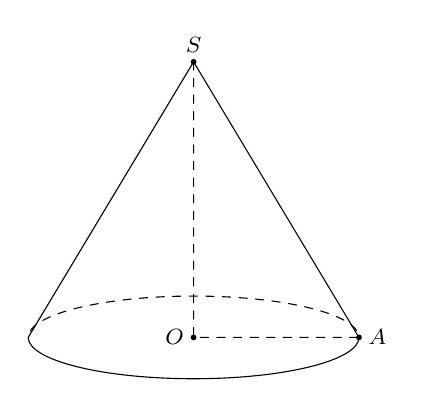
\begin{tikzpicture}[scale=.7, font=\footnotesize, line join=round, line cap=round, >=stealth]
	\def\x{3} % Bán kính trụ lớn
	\pgfmathsetmacro{\y}{\x/4} % Bán kính trục bé
	\def\h{5} % Chiều cao
	\coordinate[label=left:$O$] (O) at (0,0);
	\coordinate[label=right:$A$] (A) at (\x,0);
	\coordinate[label=above:$S$] (S) at (0,\h);
	\draw (A) arc (0:-180:{\x} and {\y})--(S)--cycle;
	\draw[dashed] (S)--(O)--(A) arc (0:180:{\x} and {\y});
	\foreach \diem in {A,S,O}	\fill (\diem)circle(1.5pt);
	\end{tikzpicture}}
}
\end{vd}
\begin{vd}%[TLDH4-Nguyễn Cao Cường]%[2H2B1-1]%Ví dụ 2.
	Cho tam giác $SOA$ vuông tại $O$ có $OA=3$ cm, $SA=5$ cm, quay tam giác $SOA$ xung quanh cạnh $SO$ được hình nón.
	\begin{itemize}
	\item[a)] Tính diện tích xung quanh và diện tích toàn phần của hình nón.
	\item[b)] Tính thể tích của khối nón tương ứng. 
	\end{itemize}
	\loigiai{
\immini{Quay tam giác $SOA$ xung quanh cạnh $SO$ được hình nón hình bên.
	\begin{itemize}
	\item[a)]Diện tích xung quanh $S_{\text{xq}}=\pi rl=15\pi$ (cm$^2$).\\
	Diện tích toàn phần $S_{\text{tp}}=\pi rl+\pi r^2=24\pi$ (cm$^2$). 
	\item[b)] Chiều cao $h=SO=\sqrt{SA^2-OA^2}=4$.\\
	Thể tích khối nón $V=\dfrac{1}{3}\pi r^2h=12\pi$ (cm$^3$).
	\end{itemize}
	}
	{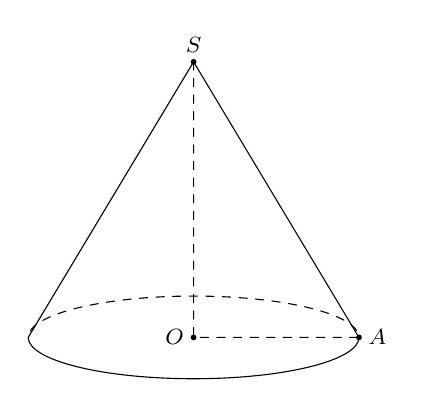
\begin{tikzpicture}[scale=.7, font=\footnotesize, line join=round, line cap=round, >=stealth]
	\def\x{3} % Bán kính trụ lớn
	\pgfmathsetmacro{\y}{\x/4} % Bán kính trục bé
	\def\h{5} % Chiều cao
	\coordinate[label=left:$O$] (O) at (0,0);
	\coordinate[label=right:$A$] (A) at (\x,0);
	\coordinate[label=above:$S$] (S) at (0,\h);
	\draw (A) arc (0:-180:{\x} and {\y})--(S)--cycle;
	\draw[dashed] (S)--(O)--(A) arc (0:180:{\x} and {\y});
	\foreach \diem in {A,S,O}	\fill (\diem)circle(1.5pt);
	\end{tikzpicture}}
}
\end{vd}
\begin{vd}%[TLDH4-Nguyễn Cao Cường]%[2H2B1-1]%Ví dụ 3.
	Cho tam giác $SAB$ đều cạnh $a$, $O$ là trung điểm của $AB$, quay tam giác $SAB$ xung quanh cạnh $SO$ được hình nón.
	\begin{itemize}
	\item[a)] Tính diện tích xung quanh và diện tích toàn phần của hình nón.
	\item[b)] Tính thể tích của khối nón tương ứng.
	\end{itemize}
	\loigiai{
\immini{Quay tam giác $SAB$ xung quanh cạnh $SO$ được hình nón như hình vẽ. Ta có $r=\dfrac{AB}{2}=\dfrac{a}{2}$.
	\begin{itemize}
	\item[a)]Diện tích xung quanh $S_{\text{xq}}=\pi rl=\dfrac{\pi a^2}{2}$.\\
	Diện tích toàn phần $S_{\text{tp}}=\pi rl+\pi r^2=\dfrac{3\pi a^2}{4}$.
	\item[b)] Chiều cao $h=SO=\dfrac{a\sqrt{3}}{2}$.\\
	Thể tích khối nón: $V=\dfrac{1}{3}\pi r^2h=\dfrac{\pi a^3\sqrt{3}}{24}$.
	\end{itemize}
	}
{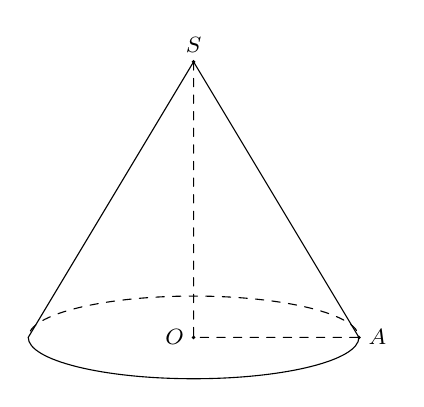
\begin{tikzpicture}[scale=.7, font=\footnotesize, line join=round, line cap=round, >=stealth]
	\def\x{3} % Bán kính trụ lớn
	\pgfmathsetmacro{\y}{\x/4} % Bán kính trục bé
	\def\h{5} % Chiều cao
	\coordinate[label=left:$O$] (O) at (0,0);
	\coordinate[label=right:$A$] (A) at (\x,0);
	\coordinate[label=above:$S$] (S) at (0,\h);
	\draw (A) arc (0:-180:{\x} and {\y})--(S)--cycle;
	\draw[dashed] (S)--(O)--(A) arc (0:180:{\x} and {\y});
	\foreach \diem in {A,S,O}	\fill (\diem)circle(1pt);
	\end{tikzpicture}	
}
}
\end{vd}
\begin{vd}%[TLDH4-Nguyễn Cao Cường]%[2H2K1-1]%Ví dụ 4.
	Cho hình chóp tứ giác đều $S.ABCD$ có cạnh đáy bằng $a$. Góc giữa mặt bên và mặt đáy bằng $60^{\circ}$. Một hình nón có đỉnh $S$ và đường tròn đáy nội tiếp tứ giác $ABCD$.
	\begin{itemize}
	\item[a)] Tính diện tích xung quanh của hình nón.
	\item[b)] Khi đó thể tích khối nón tương ứng.
	\end{itemize}
	\loigiai{
	\immini{
	Gọi $H$, $I$ lần lượt là trung điểm các đoạn $AC$ và $CD$ thì $CD\perp IH$ và $CD\perp SH\Rightarrow CD\perp SI$\\
	Do đó$\widehat{\left((SCD),(ABC)\right)}=\widehat{SIH}\Rightarrow\widehat{SIH}=60^{\circ}$.\\
	Xét tam giác $SIH$ có\\
	$\heva{&IH=\dfrac{1}{2}BC=\dfrac{a}{2}\\& SH=IH\cdot\tan\widehat{SIH}=\dfrac{a\sqrt{3}}{2}\\&SI=\dfrac{IH}{\cos{60}^{\circ}}=a.}$\\
	Hình nón nội tiếp $S.ABCD$ có bán kính $r=IH=\dfrac{a}{2}$;\\
	đường sinh $l=SI=a$; đường cao $h=SH=\dfrac{a\sqrt{3}}{2}$.}
	{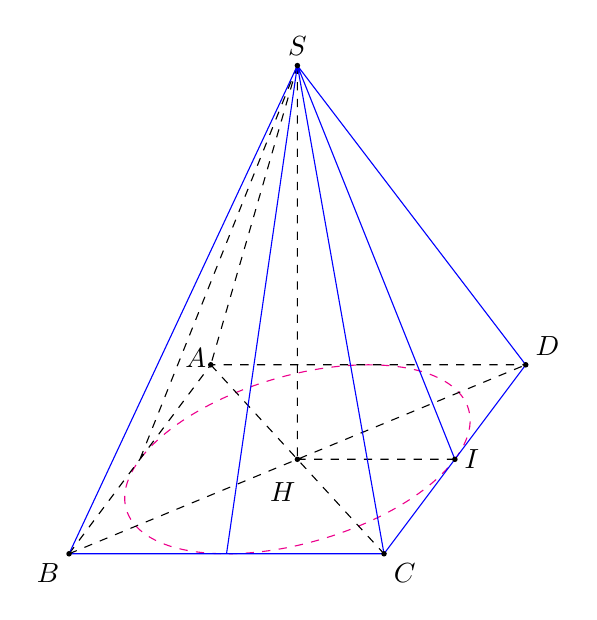
\begin{tikzpicture}
	\def\r{2}
	\def\h{5}
	\path
	(0,\h) coordinate (S) node[above]{$S$};
	\begin{scope}[xslant=.75,yscale=.6]
	\path
	(0,0) coordinate (H) +(-100:.3) node[below]{$H$}
	(-\r,\r) coordinate (A) +(150:.3) node{$A$}
	(-\r,-\r) coordinate (B) node[below left]{$B$}
	(\r,-\r) coordinate (C) node[below right]{$C$}
	(\r,\r) coordinate (D) node[above right]{$D$}
	(-\r,0) coordinate (M)
	(0,-\r) coordinate (N)
	(\r,0) coordinate (I) node[right]{$I$}
	(0,\r) coordinate (K);
	\draw[dashed,magenta] (H) circle(\r);
	\draw[dashed] (B)|-(D) (S)--(M);
	\draw[blue] (B)-|(D);
	\end{scope}
	\draw[dashed] (S)--(H) (S)--(A) (A)--(C) (B)--(D) (H)--(I);
	\draw[blue] (S)--(B) (S)--(C) (S)--(D) (S)--(I) (S)--(N);
	\foreach \diem in {A,B,C,D,S,H,I}	\fill (\diem)circle(1pt);
	\end{tikzpicture}}
\noindent 	a) Diện tích xung quanh $S_{\text{xq}}=\pi rl=\dfrac{\pi a^2}{2}$.\\
b) Thể tích hình nón đó là $V_n=\dfrac{1}{3}\pi r^2h=\dfrac{1}{3}\pi\left(\dfrac{a}{2}\right)^2\cdot\dfrac{a\sqrt{3}}{2}=\dfrac{a^3\pi\sqrt{3}}{24}$.

}
\end{vd}
\begin{vd}%[TLDH4-Nguyễn Cao Cường]%[2H2K1-5]%Ví dụ 5.
	Cho nửa đường tròn đường kính $AB=2R$ và điểm $C$ thay đổi trên nửa đường tròn đó, đặt $\alpha=\widehat{CAB}$ và gọi $H$ là hình chiếu vuông góc của $C$ lên $AB$. Tìm $\alpha$ sao cho thể tích vật thể tròn xoay tạo thành khi quay tam giác $ACH$ quanh trục $AB$ đạt giá trị lớn nhất.
	\loigiai{
\immini{Ta có $\heva{&AC=AB\cdot\cos\alpha=2R\cdot\cos\alpha\\&CH=AC\cdot\sin\alpha=2R\cdot\cos\alpha\cdot\sin\alpha\\&AH=AC\cdot\cos\alpha=2R\cdot\cos^2\alpha.}$ \\
	Thể tích vật thể tròn xoay tạo thành khi quay tam giác $ACH$ quanh trục $AB$ là\\
	$V=\dfrac{1}{3}AH\cdot\pi\cdot CH^2=\dfrac{8}{3}R^3\cdot\cos^4\alpha\cdot\sin^2\alpha$.\\
	Đặt $t=\cos^2\alpha$ với $(0<t<1)$. \\
	Khi đó 
	\allowdisplaybreaks
	\begin{eqnarray*}
	V&=&\dfrac{8}{3}R^3t^2(1-t)\\
	&=&\dfrac{8}{6}R^3\cdot t\cdot t(2-2t)\\
	&\leq&\dfrac{8}{6}R^3\left(\dfrac{t+t+2-2t}{3}\right)^3
	\end{eqnarray*}
  	Vậy $V$ lớn nhất khi $t=\dfrac{2}{3}$ khi $\alpha=\arctan\dfrac{1}{\sqrt{2}}$.}
	{	\begin{tikzpicture}[scale=.7, font=\footnotesize, line join=round, line cap=round, >=stealth]
	\path
	(0,0) coordinate (C)node[left]{$C$}
	(0,3) coordinate (A)node[above]{$A$}
	(4,0) coordinate (B)node[right]{$B$}
	(2,1.5) coordinate (O)
	;
	\coordinate[label=above right:$H$] (H) at ($(A)!(C)!(B)$) ;
	\draw (O) circle(2.5)
	(A)--(B)--(C)--cycle
	(C)--(H)
	;
	\foreach \diem in {A,B,C,H}	\fill (\diem)circle(1pt);
	\end{tikzpicture}
	\\	
	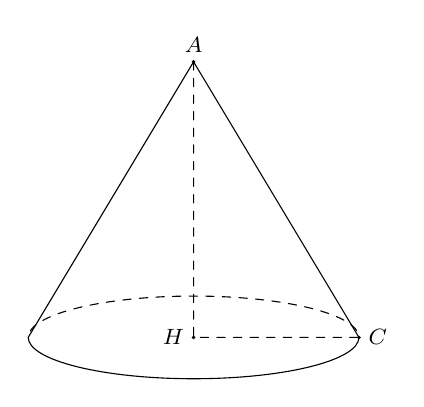
\begin{tikzpicture}[scale=.7, font=\footnotesize, line join=round, line cap=round, >=stealth]
	\def\x{3} % Bán kính trụ lớn
	\pgfmathsetmacro{\y}{\x/4} % Bán kính trục bé
	\def\h{5} % Chiều cao
	\coordinate[label=left:$H$] (O) at (0,0);
	\coordinate[label=right:$C$] (A) at (\x,0);
	\coordinate[label=above:$A$] (S) at (0,\h);
	\draw (A) arc (0:-180:{\x} and {\y})--(S)--cycle;
	\draw[dashed] (S)--(O)--(A) arc (0:180:{\x} and {\y});
	\foreach \diem in {A,S,O}	\fill (\diem)circle(1pt);
	\end{tikzpicture}
	}
}
\end{vd}
\subsubsection{Câu hỏi trắc nghiệm}
\begin{ex}%[TLDH4-Nguyễn Cao Cường]%[2H2Y1-2]%Câu 1.
	Cho hình nón đỉnh $S$ có đáy là đường tròn tâm $O$, bán kính $R$. Biết $SO=h$. Độ dài đường sinh của hình nón bằng
	\choice
	{$\sqrt{h^2-R^2}$}
	{\True $\sqrt{h^2+R^2}$}
	{$2\sqrt{h^2-R^2}$}
	{$2\sqrt{h^2+R^2}$}
	\loigiai{
	Ta có đường sinh $l=\sqrt{h^2+R^2}$.}
\end{ex}
\begin{ex}%[TLDH4-Nguyễn Cao Cường]%[2H2Y1-1]%Câu 2.
	Cho khối nón có bán kính $r=\sqrt{5}$ và chiều cao $h=3$. Tính thể tích $V$ của khối nón. 
	\choice
	{$V=9\pi\sqrt{5}$}
	{$V=3\pi\sqrt{5}$}
	{$V=\pi\sqrt{5}$}
	{\True $V=5\pi$}
	\loigiai{
	Thể tích $V$ của khối nón là $V=\dfrac{1}{3}\pi r^2h=\dfrac{1}{3}\pi 5\cdot 3=5\pi$.}
\end{ex}
\begin{ex}%[TLDH4-Nguyễn Cao Cường]%[2H2Y1-2]%Câu 3.
	Cho hình nón $(N)$ có đường kính đáy bằng $4a$, đường sinh bằng $5a$. Tính diện tích xung quanh $S$ của hình nón $(N)$. 
	\choice
	{\True $S=10\pi a^2$}
	{$S=14\pi a^2$}
	{$S=36\pi a^2$}
	{$S=20\pi a^2$}
	\loigiai{
	Diện tích xung quanh của hình nón $(N)$ là $S=\pi rl =\pi\cdot 2a\cdot 5a =10\pi a^2$.}
\end{ex}
\begin{ex}%[TLDH4-Nguyễn Cao Cường]%[2H2Y1-2]%Câu 4.
	Trong không gian cho tam giác $ABC$ vuông tại $A$, $AB=a$ và $AC=a\sqrt{3}$. Tính độ dài đường sinh $l$ của hình nón có được khi quay tam giác $ABC$ xung quanh trục $AB$. 
	\choice
	{$l=a$}
	{\True $l=2a$}
	{$l=\sqrt{3}a$}
	{$l=\sqrt{2}a$}
	\loigiai{
	\immini{
	Tam giác $ABC$ vuông tại $A$, $AB=a$ và $AC=a\sqrt{3}$ nên $BC=2a$.\\
	Độ dài đường sinh $l$ của hình nón có được khi quay tam giác $ABC$ xung quanh trục $AB$ là $l=BC=2a$.}
	{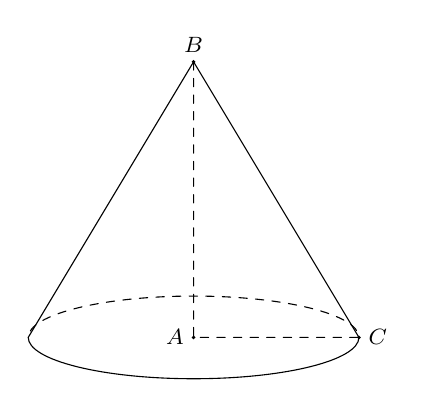
\begin{tikzpicture}[scale=.7, font=\footnotesize, line join=round, line cap=round, >=stealth]
	\def\x{3} % Bán kính trụ lớn
	\pgfmathsetmacro{\y}{\x/4} % Bán kính trục bé
	\def\h{5} % Chiều cao
	\coordinate[label=left:$A$] (A) at (0,0);
	\coordinate[label=right:$C$] (C) at (\x,0);
	\coordinate[label=above:$B$] (B) at (0,\h);
	\draw (C) arc (0:-180:{\x} and {\y})--(B)--cycle;
	\draw[dashed] (B)--(A)--(C) arc (0:180:{\x} and {\y});
	\foreach \diem in {A,B,C}	\fill (\diem)circle(1pt);
	\end{tikzpicture}}
}
\end{ex}
\begin{ex}%[TLDH4-Nguyễn Cao Cường]%[2H2Y1-2]%Câu 5.
	Trong không gian, cho tam giác $ABC$ vuông tại $A$, $AC=a$ và $BC=2a$. Tính diện tích xung quanh của hình nón, nhận được khi quay tam giác $ABC$ xung quanh trục $AB$. 
	\choice
	{\True $2\pi a^2$}
	{$\pi a^2$}
	{$4\pi a^2$}
	{$2\pi a^2\sqrt{3}$}
	\loigiai{
	\immini{Diện tích xung quanh $S_{\text{xq}}=\pi rl=2\pi a^2$.}
	{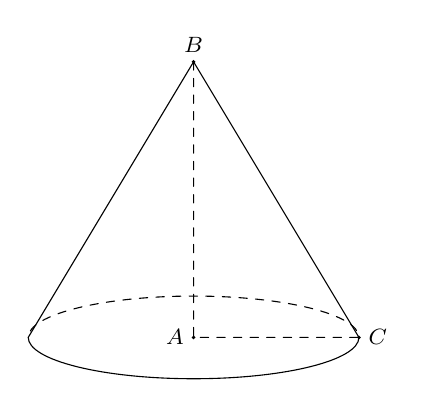
\begin{tikzpicture}[scale=.7, font=\footnotesize, line join=round, line cap=round, >=stealth]
	\def\x{3} % Bán kính trụ lớn
	\pgfmathsetmacro{\y}{\x/4} % Bán kính trục bé
	\def\h{5} % Chiều cao
	\coordinate[label=left:$A$] (A) at (0,0);
	\coordinate[label=right:$C$] (C) at (\x,0);
	\coordinate[label=above:$B$] (B) at (0,\h);
	\draw (C) arc (0:-180:{\x} and {\y})--(B)--cycle;
	\draw[dashed] (B)--(A)--(C) arc (0:180:{\x} and {\y});
	\foreach \diem in {A,B,C}	\fill (\diem)circle(1pt);
	\end{tikzpicture}}
}
\end{ex}
\begin{ex}%[TLDH4-Nguyễn Cao Cường]%[2H2B1-2]%Câu 6.
	Một hình nón có thiết diện qua trục là tam giác đều cạnh bằng $a$. Diện tích toàn phần của hình nón là 
	\choice
	{$\pi a^2$}
	{\True $\dfrac{3\pi a^2}{4}$}
	{$\dfrac{\pi a^2}{2}$}
	{$\dfrac{3\pi a^2}{2}$}
	\loigiai{
	Ta có $l=a,R=\dfrac{a}{2}$. Diện tích toàn phần $S_{\text{tp}}=\pi rl+\pi r^2=\dfrac{3\pi a^2}{4}$.}
\end{ex}
\begin{ex}%[TLDH4-Nguyễn Cao Cường]%[2H2B1-2]%Câu 7.
	Cho hình nón có độ dài đường sinh bằng đường kính đáy. Diện tích đáy của hình nón bằng $\pi$. Chiều cao của hình nón bằng
	\choice
	{\True $\sqrt{3}$}
	{$\sqrt{5}$}
	{$1$}
	{$\sqrt{2}$}
	\loigiai{
	Theo đề bài, ta có đường sinh $l=2R$.\\
	Mà $S=\pi R^2 = \pi \Leftrightarrow R=1$. Do đó $l=2$.\\
	Khi đó chiều cao $h=\sqrt{l^2-R^2}=\sqrt{4-1}=\sqrt{3}$.}
\end{ex}
\begin{ex}%[TLDH4-Nguyễn Cao Cường]%[2H2B1-2]%Câu 8.
	Cho hình nón $(N)$ có độ dài đường sinh bằng 5 và diện tích xung quanh bằng $15\pi$. Tính diện tích toàn phần của hình nón $(N)$. 
	\choice
	{$33\pi$}
	{\True $24\pi$}
	{$12\pi$}
	{$30\pi$}
	\loigiai{
	Ta có $S_{\text{xq}}=\pi rl\Rightarrow 15\pi=\pi r\cdot 5\Rightarrow r=3$.\\
	Diện tích toàn phần $S_{\text{tp}}=\pi rl+\pi r^2=24\pi$.}
\end{ex}
\begin{ex}%[TLDH4-Nguyễn Cao Cường]%[2H2B1-2]%Câu 9.
	Cho hình nón có bán kính đáy là $4a$, chiều cao là $3a$. Diện tích toàn phần hình nón bằng 
	\choice
	{\True $36\pi a^2$}
	{$72\pi a^2$}
	{$56\pi a^2$}
	{$32\pi a^2$}
	\loigiai{
	Đường sinh $l=\sqrt{r^2+h^2}=5a$.\\
	$S_{\text{tp}}=\pi rl+\pi r^2=\pi\cdot 4a\cdot 5a+\pi 16a^2=36\pi a^2$.}
\end{ex}
\begin{ex}%[TLDH4-Nguyễn Cao Cường]%[2H2B1-2]%Câu 10.
	Trong không gian cho tam giác $ABC$ vuông cân tại $A$, $AB=AC=2a$. Gọi $H$ là trung điểm của cạnh $BC$. Quay tam giác $ABC$ xung quanh trục $AH$, ta được một hình nón. Tính bán kính đáy của hình nón đó?
	\choice
	{$\dfrac{a}{2}$}
	{$a$}
	{$\dfrac{a\sqrt{2}}{2}$}
	{\True $a\sqrt{2}$}
	\loigiai{
	Ta có $BC=AB\cdot\sqrt{2}=2a\sqrt{2}\Rightarrow r=a\sqrt{2}$.}
\end{ex}
\begin{ex}%[TLDH4-Nguyễn Cao Cường]%[2H2B1-2]%Câu 11.
	Một hình nón bán kính đáy bằng $5$ (cm), góc ở đỉnh là $120^{\circ}$. Tính diện tích xung quanh của hình nón. 
	\choice
	{$\dfrac{25\pi\sqrt{3}}{2}$ (cm$^2$)}
	{$\dfrac{100\pi\sqrt{3}}{3}$ (cm$^2$)}
	{\True $\dfrac{50\pi\sqrt{3}}{3}$ (cm$^2$)}
	{$\dfrac{50\pi\sqrt{3}}{2}$ (cm$^2$)}
	\loigiai{
	Độ dài đường sinh $l=\dfrac{5}{\sin{60}^{\circ}}=\dfrac{10}{\sqrt{3}}$.\\
	Diện tích xung quanh $S_{\text{xq}}=\pi rl=\pi 5\cdot\dfrac{10}{\sqrt{3}}=\dfrac{50\pi\sqrt{3}}{3}$ (cm$^2$).}
\end{ex}
\begin{ex}%[TLDH4-Nguyễn Cao Cường]%[2H2B1-2]%Câu 12.
	Cho khối nón có bán kính đường tròn đáy bằng 10 và diện tích xung quanh bằng $120\pi$. Chiều cao h của khối nón là 
	\choice
	{$\dfrac{\sqrt{11}}{2}$}
	{$\dfrac{\sqrt{11}}{3}$}
	{\True $2\sqrt{11}$}
	{$\sqrt{11}$}
	\loigiai{
	Ta có $S_{\text{xq}}=\pi rl\Rightarrow 120\pi=\pi\cdot 10\cdot l\Rightarrow l=12$.\\
	Suy ra $h=\sqrt{l^2-r^2}=2\sqrt{11}$.}
\end{ex}
\begin{ex}%[TLDH4-Nguyễn Cao Cường]%[2H2B1-1]%Câu 13.
	Trong không gian, cho tam giác vuông $OIM$ vuông tại $I$, góc $\widehat{IOM}=30^{\circ}$ và cạnh $IM=a$. Khi quay tam giác $OIM$ quanh cạnh góc vuông $OI$ thì đường gấp khúc $OIM$ tạo thành một hình nón tròn xoay. Thể tích của khối nón tròn xoay được tạo nên bởi hình nón là 
	\choice
	{$\pi a^3\sqrt{3}$}
	{$\dfrac{a^3\sqrt{3}}{3}$}
	{$\dfrac{\pi a^3\sqrt{3}}{3}$}
	{\True $\dfrac{\pi a^3\sqrt{3}}{2}$}
	\loigiai{
	\immini{
	Ta có $\triangle IOM$ vuông tại $I$ có $\widehat{IOM}=30^{\circ}\Rightarrow OI=\dfrac{IM}{\tan{30}^{\circ}}=\dfrac{a}{\dfrac{\sqrt{3}}{3}}=a\sqrt{3}$.\\
	Vậy thể tích khối nón $V=\dfrac{1}{3}\pi r^2h=\dfrac{\pi a^3\sqrt{3}}{3}$.}
	{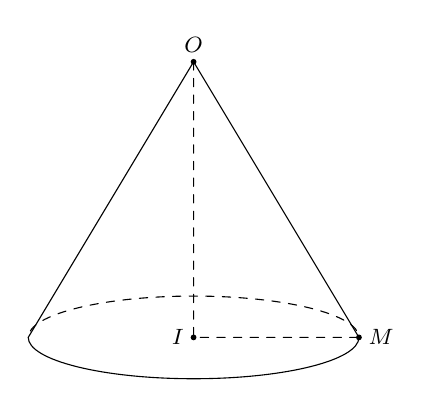
\begin{tikzpicture}[scale=.7, font=\footnotesize, line join=round, line cap=round, >=stealth]
	\def\x{3} % Bán kính trụ lớn
	\pgfmathsetmacro{\y}{\x/4} % Bán kính trục bé
	\def\h{5} % Chiều cao
	\coordinate[label=left:$I$] (I) at (0,0);
	\coordinate[label=right:$M$] (M) at (\x,0);
	\coordinate[label=above:$O$] (O) at (0,\h);
	\draw (M) arc (0:-180:{\x} and {\y})--(O)--cycle;
	\draw[dashed] (O)--(I)--(M) arc (0:180:{\x} and {\y});
	\foreach \diem in {M,I,O}	\fill (\diem)circle(1.5pt);
	\end{tikzpicture}
	}
}
\end{ex}
\begin{ex}%[TLDH4-Nguyễn Cao Cường]%[2H2B1-1]%Câu 14.
	Trong không gian, cho tam giác vuông $ABC$ tại $B$ có $AB=1$, $\widehat{BAC}=60^{\circ}$. Quay tam giác đó xung quanh trục $AB$ ta được một hình nón. Tính thể tích khối nón đó. 
	\choice
	{\True $\pi$}
	{$2\pi$}
	{$3\pi$}
	{$4\pi$}
	\loigiai{
	\immini{Ta có $CB=AB\tan 60^{\circ}=\sqrt{3}$.\\ Vậy $V=\dfrac{1}{3}\pi R^2h=\dfrac{1}{3}\pi\cdot 3\cdot 1=\pi$.}
	{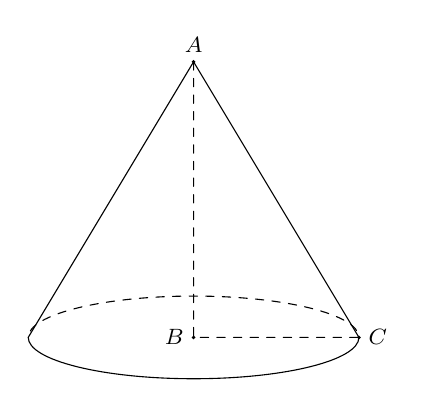
\begin{tikzpicture}[scale=.7, font=\footnotesize, line join=round, line cap=round, >=stealth]
	\def\x{3} % Bán kính trụ lớn
	\pgfmathsetmacro{\y}{\x/4} % Bán kính trục bé
	\def\h{5} % Chiều cao
	\coordinate[label=left:$B$] (B) at (0,0);
	\coordinate[label=right:$C$] (C) at (\x,0);
	\coordinate[label=above:$A$] (A) at (0,\h);
	\draw (C) arc (0:-180:{\x} and {\y})--(A)--cycle;
	\draw[dashed] (A)--(B)--(C) arc (0:180:{\x} and {\y});
	\foreach \diem in {A,B,C}	\fill (\diem)circle(1pt);
	\end{tikzpicture}}
}
\end{ex}
\begin{ex}%[TLDH4-Nguyễn Cao Cường]%[2H2B1-4]%Câu 15.
\immini{	Có một chiếc cốc có dạng như hình vẽ, biết chiều cao của chiếc cốc là $8$ cm, bán kính đáy cốc là $3$ cm, bán kính miệng cốc là $6$ cm. Tính thể tích $V$ của chiếc cốc. 
	\choice
	{$72\pi$ cm$^3$}
	{$48\pi$ cm$^3$}
	{\True$168\pi$ cm$^3$}
	{$36\pi$ cm$^3$}}
{\begin{tikzpicture}[line join=round,scale=.6]
	\draw[dashed] (0:0) arc(180:0:{1.5} and {.5});
	\draw (0:0) arc(180:360:{1.5} and {.5});
	\draw (1.5,6) ellipse ({3} and {1.5});
	\draw[name path=a](0,0)--(-1.5,6);
	\draw[name path=b](3,0)--(4.5,6);
	\end{tikzpicture}}
	\loigiai{
	Áp dụng công thức tính thể tích hình nón cụt.\\
	$V=\dfrac{\pi h}{3}\left(R^2+r^2+R\cdot r\right)=\dfrac{8\pi}{3}\left(6^2+3^2+6\cdot 3\right)=168\pi$ cm$^3$.}
\end{ex}
\begin{ex}%[TLDH4-Nguyễn Cao Cường]%[2H2B1-3]%Câu 16.
	Cho hình hộp chữ nhật $ABCD.A'B'C'D'$ có đáy là hình vuông cạnh $a$ và cạnh bên bằng $2a$. Diện tích xung quanh $S_{\text{xq}}$ của hình nón có đỉnh là tâm $O$ của hình vuông $A'B'C'D'$ và đáy là hình tròn nội tiếp hình vuông $ABCD$ là 
	\choice
	{\True $S_{\text{xq}}=\dfrac{\pi a^2\sqrt{17}}{4}$}
	{$S_{\text{xq}}=\pi a^2$}
	{$S_{\text{xq}}=\dfrac{\pi a^2\sqrt{17}}{2}$}
	{$S_{\text{xq}}=\pi a^2\sqrt{17}$}
	\loigiai{
	\immini{Dựa vào giả thiết ta có bán kính đáy hình nón là bán kính đường tròn nội tiếp hình vuông nên $r=\dfrac{a}{2}$.\\
	Chiều cao hình nón là khoảng cách từ $O$ đến mặt phẳng $(ABCD)$ nên $h=2a$.\\
	Độ dài đường sinh hình nón là $$l=\sqrt{h^2+r^2}=\sqrt{4a^2+\dfrac{a^2}{4}}=\dfrac{a\sqrt{17}}{2}$$.\\
	Diện tích xung quanh của hình nón là $S_{\text{xq}}=\pi rl=\pi\dfrac{a}{2}\cdot\dfrac{a\sqrt{17}}{2}=\dfrac{\pi a^2\sqrt{17}}{4}$.}
	{\begin{tikzpicture}[line join=round]
	\def\r{2} % bán kính đáy
	\def\h{4.5} % chiều cao
	% Đáy dưới
	\begin{scope}[yscale=.3,xslant=.3]
	\draw[dashed] (0,0) circle(\r);
	\draw
	(-\r,-\r) coordinate (A)node[below]{$A$}
	--(\r,-\r) coordinate (B)node[below]{$B$} node[below,midway]{$a$}
	--(\r,\r) coordinate (C)node[right]{$C$} node[right=1mm,pos=.4]{$a$}
	(-\r,\r) coordinate (D)node[above right]{$D$}
	(-\r,0) coordinate (L)
	(\r,0) coordinate (R);
	\draw[dashed] (D)--(A) (D)--(C);
	\end{scope}
	% Đáy trên
	\begin{scope}[yshift=\h cm,yscale=.3,xslant=.3]
	\draw 
	%(0,0) circle(\r)
	(-\r,-\r) coordinate (At)node[left]{$A'$}
	--(\r,-\r) coordinate (Bt)node[right]{$B'$}
	--(\r,\r) coordinate (Ct)node[right]{$C'$}
	--(-\r,\r) coordinate (Dt)node[above right]{$D'$}--cycle
	;
	%(-\r,0) coordinate (Lt)
	%(\r,0) coordinate (Rt)
	\coordinate [label=above:$O$](O)at ($(At)!.5!(Ct)$)
	;
	\end{scope}
	\draw[dashed] (D)--(Dt) (L)--(O)--(R)--cycle
	%(L)--(Lt)
	;
	\draw (A)--(At) node[left,midway]{$2a$}
	(B)--(Bt)--(Dt) (C)--(Ct)--(At) 
	%(R)--(Rt)
	;
	\end{tikzpicture}}
}
\end{ex}
\begin{ex}%[TLDH4-Nguyễn Cao Cường]%[2H2K1-2]%Câu 17.
	Cho hình nón tròn xoay có chiều cao $h=20$ cm, bán kính đáy $r=25$ cm. Mặt phẳng $(\alpha)$ đi qua đỉnh của hình nón cách tâm của đáy $12$ cm. Tính diện tích thiết diện của hình nón cắt bởi mp $(\alpha)$. 
	\choice
	{$S=400$ (cm$^2$)}
	{$S=406$ (cm$^2$)}
	{$S=300$ (cm$^2$)}
	{\True $S=500$ (cm$^2$)}
	\loigiai{
	\immini{
	Ta có $\mathrm{d}\left(I,(\alpha)\right)=IH=12$.\\
	Diện tích thiết diện của hình nón cắt bởi mặt phẳng $(\alpha)$ là $S_{\triangle SAB}=\dfrac{1}{2}SJ\cdot AB$.\\
	Trong tam giác $SIJ$ vuông tại $I$ $$\dfrac{1}{IH^2}=\dfrac{1}{SI^2}+\dfrac{1}{IJ^2}\Leftrightarrow\dfrac{1}{{12}^2}=\dfrac{1}{{20}^2}+\dfrac{1}{IJ^2}\Leftrightarrow IJ=15$$.\\
	Suy ra $SJ=\sqrt{SI^2+IJ^2}=\sqrt{{20}^2+{15}^2}=25$.\\
	Mặt khác ta có $J$ là trung điểm của $AB$ và $IJ\perp AB$.\\
	Xét tam giác $IAJ$ vuông tại $J$ có\\ $JA=\sqrt{IA^2-IJ^2}=\sqrt{{25}^2-{15}^2}=20$.\\
	Vậy $S_{\triangle SAB}=\dfrac{1}{2}SJ\cdot AB=25\cdot 20=500$ (cm$^2$).}
	{\begin{tikzpicture}[line join=round,scale=.7]
	\draw[dashed] (0:0) arc(180:0:{3} and {.9});
	\draw (0:0) arc(180:360:{3} and {.9});
	\coordinate (S) at (3,6);
	\coordinate (I) at (3,0);
	\coordinate (M) at (0,0);
	\coordinate (N) at (6,0);
	\path (M) arc (180:-75:{3} and {.9})coordinate (A);
	\path (M) arc (180:40:{3} and {.9})coordinate (B);
	\coordinate (J) at (intersection of A--B and M--N);
	\coordinate (H) at ($(S)!.7!(J)$) ;
	\draw (M)--(S)--(N) (S)--(A);
	\draw[dashed] (S)--(I)--(J)(S)--(J)(S)--(B)--(A)(I)--(H);
	\begin{scope}
	\clip (A)--(S)--(B);
	\draw (S) circle (1.5);
	\end{scope}
	\foreach \d/\g in{S/90,I/130,J/-80,A/-90,B/-90,H/180}
	\draw[fill=black](\d)circle(2pt)node[shift={(\g:0.35)}]{$\d$};
	\end{tikzpicture}}
}
\end{ex}
\begin{ex}%[TLDH4-Nguyễn Cao Cường]%[2H2B1-1]%Câu 18.
	Cho hình nón có góc ở đỉnh bằng $60^{\circ},$ diện tích xung quanh bằng $6\pi a^2$. Tính thể tích $V$ của khối nón đã cho. 
	\choice
	{$V=\dfrac{3\pi a^3\sqrt{2}}{4}$}
	{$V=\dfrac{\pi a^3\sqrt{2}}{4}$}
	{\True$V=3\pi a^3$}
	{$V=\pi a^3$}
	\loigiai{
	\immini{
	Thể tích $V=\dfrac{1}{3}\pi R^2h=\dfrac{1}{3}\pi\cdot OA^2\cdot SO$.\\
	Ta có $\widehat{ASB}=60^{\circ}\Rightarrow\widehat{ASO}=30^{\circ}\Rightarrow\tan 30^{\circ}=\dfrac{OA}{SO}=\dfrac{1}{\sqrt{3}}\Rightarrow SO=OA\sqrt{3}$.\\
	Lại có $S_{\text{xq}}=\pi Rl=\pi\cdot OA\cdot SA=\pi\cdot OA\sqrt{OA^2+SO^2}=6\pi a^2$ \\
	$ \Rightarrow OA\sqrt{OA^2+3OA^2}=6a^2\Rightarrow 2OA^2=6a^2\Rightarrow OA=a\sqrt{3}\Rightarrow SO=3a\Rightarrow V=\dfrac{1}{3}\pi\cdot 3a^2\cdot 3a=3\pi a^3 $.}
	{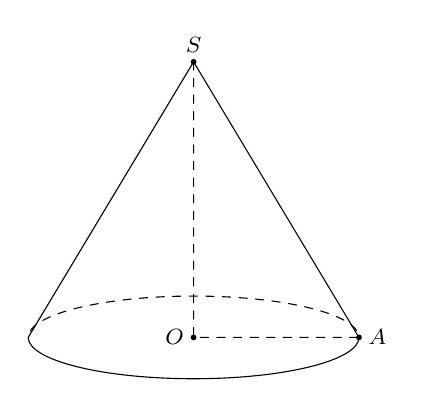
\begin{tikzpicture}[scale=.7, font=\footnotesize, line join=round, line cap=round, >=stealth]
	\def\x{3} % Bán kính trụ lớn
	\pgfmathsetmacro{\y}{\x/4} % Bán kính trục bé
	\def\h{5} % Chiều cao
	\coordinate[label=left:$O$] (I) at (0,0);
	\coordinate[label=right:$A$] (M) at (\x,0);
	\coordinate[label=above:$S$] (O) at (0,\h);
	\draw (M) arc (0:-180:{\x} and {\y})--(O)--cycle;
	\draw[dashed] (O)--(I)--(M) arc (0:180:{\x} and {\y});
	\foreach \diem in {M,I,O}	\fill (\diem)circle(1.5pt);
	\end{tikzpicture}}
}
\end{ex}
\begin{ex}%[TLDH4-Nguyễn Cao Cường]%[2H2K1-3]%Câu 19.
	Cho hình nón đỉnh $S$, đáy là đường tròn nội tiếp tam giác $ABC$. Biết rằng $AB=BC=10a$, $AC=12a$, góc tạo bởi hai mặt phẳng $(SAB)$ và $(ABC)$ bằng $45^{\circ}$. Tính thể tích $V$ của khối nón đã cho. 
	\choice
	{$V=3\pi a^3$}
	{\True $V=9\pi a^3$}
	{$V=27\pi a^3$}
	{$V=12\pi a^3$}
	\loigiai{
	\immini{
	Gọi $O$ là tâm đường tròn nội tiếp tam giác $ABC$. Hạ $OH\perp AB$, khi đó góc tạo bởi hai mặt phẳng $(SAB)$ và $(ABC)$ chính là $\widehat{SHO}=45^{\circ}$ nên $OH=SO=r=h$.\\
	Lại có $S_{\triangle ABC}=p\cdot r\Rightarrow r=\dfrac{S_{\triangle ABC}}{p}$.\\
	Tính được $p=16a$, $S_{\triangle ABC}=\sqrt{p(p-a)(p-b)(p-c)}=48a^2$.\\
	Suy ra $r=3a$. Vậy $V=\dfrac{1}{3}\pi r^2h=\dfrac{1}{3}\pi(3a)^3=9\pi a^3$.}
	{	\begin{tikzpicture}[scale=1, font=\footnotesize, line join=round, line cap=round,yscale=0.6]
	\def\noitiep(#1,#2,#3)(#4,#5){
	\path
	($($(#2)!2mm!(#1)$)!0.5!($(#2)!2mm!(#3)$)$) coordinate (#2a)
	($($(#1)!2mm!(#2)$)!0.5!($(#1)!2mm!(#3)$)$) coordinate (#1a)
	(intersection of #2-- #2a and #1--#1a) coordinate (#4)
	($(#1)!(#4)!(#2)$) coordinate (pro);
	\path let \p1 =($(#4)-(pro)$),
	\n1= {scalar(veclen(\x1,\y1)/1cm)}
	in \pgfextra{\xdef#5{\n1}};
	}
	\path 
	(0,0) coordinate (C)
	(3.5,-4) coordinate (B)
	(4.5,0) coordinate (A) 
	;
	\noitiep(A,B,C)(O,\r)
	\path 
	($(O)+(0,5)$)coordinate (S)
	($(A)!(O)!(B)$) coordinate (H)
	($(O)+(0:\r)$) coordinate (E)
	($(O)+(180:\r)$) coordinate (F)
	;
	\draw[dashed] (O) circle (\r);	
	\draw (B)--(A)--(S)--(B)--(C)--(S)--(H);
	\draw [dashed] (A)--(C) (S)--(F) (S)--(O)--(H);
	\foreach \p/\g in {S/90,A/0,B/-90,C/180,H/350,O/160}\draw[fill=black] (\p) circle (1pt)node[shift={(\g:.3)}]{$\p$};
	\end{tikzpicture}}
	}
\end{ex}
%%%%%%%
\begin{ex}%[2H2B1-1]%Câu 13.
	Cho hình lập phương $ABCD.A'B'C'D'$ có cạnh bằng $a$. Gọi $(C)$ và $(C')$ lần lượt là hai đường tròn ngoại tiếp hình vuông $ABCD$ và $A'B'C'D'$. Hình trụ có hai đáy là $(C)$ và $(C')$ có thể tích là
	\choice
	{$\dfrac{1}{3}\pi a^3$}
	{$2\pi a^3$}
	{$\pi a^3$}
	{\True $\dfrac{\pi a^3}{2}$}
	\loigiai{
		\immini{
			Ta có bán kính đáy hình trụ là $r=\dfrac{A'C'}{2}=\dfrac{a\sqrt{2}}{2}$.\\
			Đường cao là $h=a$. Khi đó $V=\pi r^2h=\dfrac{\pi a^3}{2}$.
		}{
			\begin{tikzpicture}[scale=0.7, font=\footnotesize, line join=round, line cap=round, >=stealth]
			\def \x{3} %bán kính trục lớn elip
			\def \y{1} %bán kính trục bé elip
			\def \h{3.5} %chiều cao hình trụ
			\coordinate (M) at (0,0);
			\coordinate (N) at (2*\x,0);
			\coordinate (O) at ($(M)!0.5!(N)$);
			\coordinate (O') at ($(O)+(0,\h)$);
			\coordinate (M') at ($(M)+(0,\h)$);
			\coordinate (N') at ($(N)+(0,\h)$);
			\draw[dashed] (N) arc(0:180:\x cm and \y cm);
			\draw (N) arc(0:-180:\x cm and \y cm);
			\draw (O') ellipse (\x cm and \y cm);
			\coordinate (A) at ($(O)+(112:\x cm and \y cm)$);
			\coordinate (B) at ($(O)+(42:\x cm and \y cm)$);
			\coordinate (C) at ($(O)!-1!(A)$);
			\coordinate (D) at ($(O)!-1!(B)$);
			\tkzDefPointsBy[translation=from O to O'](A,B,C,D){A'}{B'}{C'}{D'}
			\tkzDrawPolygon(A',B',C',D')
			\tkzDrawPolygon[dashed](A,B,C,D)
			\tkzDrawSegments(M,M' N,N' D,D' C,C')
			\tkzDrawSegments[dashed](O,O' A,C B,D A,A' B,B')
			\tkzDrawPoints[fill=black,size=3](O,O',A,B,C,D,A',B',C',D')
			\tkzLabelPoints[above](O',A',B',C',D')
			\tkzLabelPoints[below](O)
			\tkzLabelPoints[below left](D)
			\tkzLabelPoints[below right](C)
			\tkzLabelPoints[above right](B)
			\tkzLabelPoints[above left](A)
			\end{tikzpicture}
		}
	}
\end{ex}
\begin{ex}%[2H2B2-6]%Câu 14.
	Một khối cầu bán kính $R$ và một khối trụ có bán kính $R$, chiều cao $2R$. Tỉ số thể tích giữa khối cầu và khối trụ bằng
	\choice
	{$\dfrac{1}{2}$}
	{\True $\dfrac{2}{3}$}
	{$\dfrac{3}{2}$}
	{$2$}
	\loigiai{
		Thể tích của hình trụ là $V_{ht}=\pi R^2h=\pi\cdot R^2\cdot 2R=2\pi R^3$.\\
		Thể tích của khối cầu là $V_{mc}=\dfrac{4}{3}\pi R^3$. Suy ra $\dfrac{V_{mc}}{V_{ht}}=\dfrac{\dfrac{4}{3}\pi R^3}{2\pi R^3}=\dfrac{2}{3}$.}
\end{ex}
\begin{ex}%[2H2B1-1]%Câu 15.
	Cho lăng trụ tam giác đều có tất cả các cạnh bằng $a$. Một hình trụ tròn xoay có hai đáy là hai hình tròn ngoại tiếp hai đáy của lăng trụ. Thể tích của khối trụ tròn xoay bằng
	\choice
	{$\pi a^3$}
	{$\dfrac{\pi a^3}{9}$}
	{$3\pi a^3$}
	{\True $\dfrac{\pi a^3}{3}$}
	\loigiai{
		Gọi $R$, $h$ là bán kính đáy và chiều cao của hình trụ.\\
		Ta có $h=a$ (cùng đường cao với lăng trụ) và $R=\dfrac{a\sqrt{3}}{3}$ vì $R$ cũng là bán kính đường tròn ngoại tiếp đáy lăng trụ.\\
		$\Rightarrow V=\pi R^2h=\dfrac{\pi a^3}{3}$.}
\end{ex}
\begin{ex}%[2H2B1-1]%Câu 16.
	Một hình trụ có diện tích xung quanh bằng $4\pi$ và có thiết diện qua trục là hình vuông. Thể tích khối trụ tương ứng bằng
	\choice
	{\True $2\pi$}
	{$\pi$}
	{$3\pi$}
	{$4\pi$}
	\loigiai{
		Thiết diện qua trục là hình vuông nên $h=2R$.\\
		Ta có $S_{\text{xq}}=4\pi \Leftrightarrow 2\pi Rh=4\pi \Leftrightarrow \pi h^2=4\pi$.\\
		Suy ra $\heva{&h=2\\&R=1}\Rightarrow V=\pi R^2h=2\pi$.}
\end{ex}
\begin{ex}%[2H2B2-6]%Câu 17.
	Trong một chiếc hộp hình trụ người ta bỏ vào đó ba quả banh tennis, biết rằng đáy của hình trụ bằng hình tròn lớn trên quả banh và chiều cao của hình trụ bằng $3$ lần đường kính của quả banh. Gọi $S_1$ là tổng diện tích của ba quả banh và $S_2$ là diện tích xung quanh của hình trụ. Tỉ số $\dfrac{S_1}{S_2}$ bằng
	\choice
	{\True $1$}
	{$2$}
	{$3$}
	{$\dfrac{1}{2}$}
	\loigiai{
		Gọi $R$ là bán kính của $1$ quả banh.\\
		$\Rightarrow$ Tổng diện tích $3$ quả banh là $S_1=3\cdot 4\pi R^2=12\pi R^2$.\\
		Chiếc hộp có bán kính đáy cũng bằng R và chiều cao bằng $h=6R$ \\
		$ \Rightarrow $ Diện tích xung quanh hình trụ $S_2=2\pi Rh=12\pi R^2$.\\
		Vậy $\dfrac{S_1}{S_2}=1$.}
\end{ex}
\begin{ex}%[2H2B1-1]%Câu 18.
	Cắt hình trụ $(T)$ bằng một mặt phẳng song song với trục và cách trục một khoảng bằng $2$ cm được thiết diện là một hình vuông có diện tích bằng $16$ cm$^2$. Thể tích của $(T)$ là
	\choice
	{\True $32\pi$ (cm$^3$)}
	{$16\pi$ (cm$^3$)}
	{$64\pi$ (cm$^3$)}
	{$8\pi$ (cm$^3$)}
	\loigiai{
		\immini{
			Giả sử thiết diện là hình vuông $MNPQ$ như hình vẽ.\\
			Ta có $O'H=2$ và $S_{MNPQ}=PQ^2=16\Leftrightarrow PQ=4$.\\
			Khi đó $O'Q=\sqrt{O'H^2+\left(\dfrac{PQ}{2}\right)^2}=2\sqrt{2}$.\\
			Mà $h=MQ=4$.\\
			Suy ra $V_{(t)}=\pi r^2 h=\pi\cdot 8\cdot 4=32\pi$ (cm$^3$).
		}{
			\begin{tikzpicture}[scale=0.7, font=\footnotesize, line join=round, line cap=round, >=stealth]
			\def \x{2.5} %bán kính trục lớn elip
			\def \y{1} %bán kính trục bé elip
			\def \h{-3.5} %chiều cao hình trụ
			\coordinate (A) at (0,0);
			\coordinate (B) at (2*\x,0);
			\coordinate (O) at ($(A)!0.5!(B)$);
			\coordinate (O') at ($(O)+(0,\h)$);
			\coordinate (D) at ($(A)+(0,\h)$);
			\coordinate (C) at ($(B)+(0,\h)$);
			%Lấy các điểm M,N trên elip
			\coordinate (M) at ($(O)+({\x*cos(105)},{\y*sin(105)})$);
			\coordinate (N) at ($(O)+({\x*cos(32)},{\y*sin(32)})$);
			\coordinate (P) at ($(N)+(0,\h)$);
			\coordinate (Q) at ($(M)+(0,\h)$);
			\coordinate (H) at ($(P)!0.5!(Q)$);
			\draw[dashed] (C) arc(0:180:\x cm and \y cm);
			\draw (C) arc(0:-180:\x cm and \y cm);
			\draw (O) ellipse (\x cm and \y cm);
			\tkzDrawSegments(A,D B,C M,N A,B)
			\tkzDrawSegments[dashed](O,O' M,Q P,Q P,N O',P O',Q O',H C,D)
			\tkzDrawPoints[fill=black,size=3](A,B,O,O',D,C,M,N,P,Q,H)
			\tkzLabelPoints[above](O,M,N)
			\tkzLabelPoints[below](O',P)
			\tkzLabelPoints[left](A,D)
			\tkzLabelPoints[right](B,C)
			\tkzLabelPoints[below left](Q)
			\tkzLabelPoints[above right](H)
			\end{tikzpicture}
		}
	}
\end{ex}
\begin{ex}%[2H2B1-1]%Câu 19.
	Một hình trụ tròn xoay có bán kính $R=1$. Trên $2$ đường tròn $(O)$ và $(O')$ lấy lần lượt $2$ điểm $A$ và $B$ sao cho $AB=2$, góc giữa $AB$ và trục $OO'$ bằng $30^{\circ}$. Xét hai mệnh đề sau:\\
	(I) Khoảng cách giữa $OO'$ và $AB$ bằng $\dfrac{\sqrt{3}}{2}$. \\
	(II) Thể tích của hình trụ là $V=\sqrt{3}$. 
	\choice
	{\True Chỉ (I) đúng}
	{Chỉ (II) đúng}
	{Cả hai đúng}
	{Cả hai sai}
	\loigiai{
		\immini{
			Kẻ đường sinh $BC$ thì $OO'\parallel (ABC)$.\\
			Vì $(ABC)\perp(OAC)$ nên kẻ $OH\perp AC$ thì $OH\perp(ABC)$.\\
			Vậy $\mathrm{d}(OO',AB)=OH$.\\
			Trong $\triangle ABC$ có $BC=AB\cdot\cos 30^{\circ}=\sqrt{3}$, $AC=AB\cdot\sin 30^{\circ}=1$.\\
			Suy ra $\triangle OAC$ đều có cạnh bằng $1$ $\Rightarrow OH=\dfrac{\sqrt{3}}{2}$ (mệnh đề (I) đúng).\\
			Lại có $V=\pi r^2h=\pi\sqrt{3}$ (mệnh đề (II) sai).
		}{
			\begin{tikzpicture}[scale=0.7, font=\footnotesize, line join=round, line cap=round, >=stealth]
			\def \x{2.5} %bán kính trục lớn elip
			\def \y{1} %bán kính trục bé elip
			\def \h{3.5} %chiều cao hình trụ
			\coordinate (M) at (0,0);
			\coordinate (N) at (2*\x,0);
			\coordinate (O) at ($(M)!0.5!(N)$);
			\coordinate (O') at ($(O)+(0,\h)$);
			\coordinate (M') at ($(M)+(0,\h)$);
			\coordinate (N') at ($(N)+(0,\h)$);
			%Lấy các điểm A,C trên elip
			\coordinate (A) at ($(O)+({\x*cos(-80)},{\y*sin(-80)})$);
			\coordinate (C) at ($(O)+({\x*cos(-30)},{\y*sin(-30)})$);
			\coordinate (B) at ($(C)+(0,\h)$);
			\coordinate (H) at ($(A)!0.5!(C)$);
			\draw[dashed] (N) arc(0:180:\x cm and \y cm);
			\draw (N) arc(0:-180:\x cm and \y cm);
			\draw (O') ellipse (\x cm and \y cm);
			\tkzDrawSegments(M,M' N,N' B,C)
			\tkzDrawSegments[dashed](O,O' A,B A,C O,A O,C O,H)
			\tkzDrawPoints[fill=black,size=3](O,O',A,B,C,H)
			\tkzLabelPoints[above](B)
			\tkzLabelPoints[below](A,C,H)
			\tkzLabelPoints[left](O,O')
			\end{tikzpicture}
		}
	}
\end{ex}
\begin{ex}%[2H2B1-3]%Câu 20.
	Cho khối lăng trụ đứng $ABC.A'B'C'$ có đáy $ABC$ là tam giác vuông cân tại $A$, có $AB=a$; đường chéo $BC'$ của mặt bên $BB'C'C$ tạo với mặt bên $AA'C'C$ một góc $30^{\circ}$. Khối trụ ngoại tiếp lăng trụ có thể tích là
	\choice
	{\True $\dfrac{\pi a^3\cdot\sqrt{2}}{2}$}
	{$\pi a^3\cdot\sqrt{2}$}
	{$\dfrac{\pi a^3\cdot\sqrt{2}}{4}$}
	{$\dfrac{\pi a^3\cdot\sqrt{2}}{6}$}
	\loigiai{
		\immini{
			Khối trụ ngoại tiếp lăng trụ có bán kính đáy $R=\dfrac{BC}{2}=\dfrac{a\sqrt{2}}{2}$.\\
			Từ $\widehat{AC'B}=30^{\circ}\Rightarrow AC'=a\sqrt{3}\Rightarrow CC'=a\sqrt{2}$.\\
			$\Rightarrow$ Khối trụ ngoại tiếp lăng trụ có bán kính đáy $R=\dfrac{a\sqrt{2}}{2}$ và chiều cao $h=CC'=a\sqrt{2}$.\\
			Vậy thể tích $V=\dfrac{\pi a^3\cdot\sqrt{2}}{2}$.
		}{
			\begin{tikzpicture}[scale=0.7, font=\footnotesize, line join=round, line cap=round, >=stealth]
			\def \x{2} %bán kính trục lớn elip
			\def \y{1} %bán kính trục bé elip
			\def \h{3.5} %chiều cao hình trụ
			\coordinate (B) at (0,0);
			\coordinate (C) at (2*\x,0);
			\coordinate (O) at ($(B)!0.5!(C)$);
			\coordinate (O') at ($(O)+(0,\h)$);
			\coordinate (B') at ($(B)+(0,\h)$);
			\coordinate (C') at ($(C)+(0,\h)$);
			\coordinate (A) at ($(O)+({\x*cos(-75)},{\y*sin(-75)})$);
			\coordinate (A') at ($(A)+(0,\h)$);
			\draw[dashed] (C) arc(0:180:\x cm and \y cm);
			\draw (C) arc(0:-180:\x cm and \y cm);
			\draw (O') ellipse (\x cm and \y cm);
			\tkzDrawSegments(C,C' B,B' A,A' B',C' A',B' A',C')
			\tkzDrawSegments[dashed](O,O' A,B A,C B,C C',B C',A)
			\tkzDrawPoints[fill=black,size=3](A,B,O,O',A',B',C,C')
			\tkzLabelPoints[above](O',A')
			\tkzLabelPoints[below](O,A)
			\tkzLabelPoints[left](B,B')
			\tkzLabelPoints[right](C,C')
			\end{tikzpicture}
		}
	}
\end{ex}
\begin{ex}%[2H2B1-2]%Câu 21.
	Một hình trụ có bán kính đáy $r=5$ cm và khoảng cách giữa hai đáy $h=7$ cm. Cắt khối trụ bởi một mặt phẳng song song với trục và cách trục $3$ cm. Diện tích của thiết diện được tạo thành là 
	\choice
	{\True $S=56$ (cm$^2$)}
	{$S=55$ (cm$^2$)}
	{$S=53$ (cm$^2$)}
	{$S=46$ (cm$^2$)}
	\loigiai{
		\immini{
			Gọi $O$, $O'$ là tâm của hai đáy của hình trụ và $(P)$ là mặt phẳng song song với trục và cách trục $OO'$ một khoảng $3$ cm.\\
			Mặt phẳng $(P)$ cắt hai hình tròn đáy $(O)$, $(O')$ theo hai dây cung lần lượt là $AB$, $CD$ và cắt mặt xung quanh theo hai đường sinh là $AD$, $BC$.\\
			$\Rightarrow ABCD$ là hình chữ nhật.\\
			Gọi $H$ là trung điểm của $AB$.\\
			Ta có $OH\perp AB$; $OH\perp AD\Rightarrow OH\perp(ABCD)$ \\
			$ \Rightarrow\mathrm{d}\left(OO',(P)\right)=\mathrm{d}\left(O,(ABCD)\right)=OH=3$ cm.\\
			Khi đó $AB=2AH=2\sqrt{OA^2-OH^2}=8$; $AD=OO'=h=7$.\\
			Diện tích hình chữ nhật $ABCD$ là $S_{ABCD}=AB\cdot AD=56$ (cm$^2$).
		}{
			\begin{tikzpicture}[scale=0.7, font=\footnotesize, line join=round, line cap=round, >=stealth]
			\def \x{2.5} %bán kính trục lớn elip
			\def \y{1} %bán kính trục bé elip
			\def \h{3.5} %chiều cao hình trụ
			\coordinate (M) at (0,0);
			\coordinate (N) at (2*\x,0);
			\coordinate (O') at ($(M)!0.5!(N)$);
			\coordinate (O) at ($(O')+(0,\h)$);
			\coordinate (M') at ($(M)+(0,\h)$);
			\coordinate (N') at ($(N)+(0,\h)$);
			\coordinate (C) at ($(O')+({\x*cos(35)},{\y*sin(35)})$);
			\coordinate (D) at ($(O')+({\x*cos(-75)},{\y*sin(-75)})$);
			\coordinate (B) at ($(C)+(0,\h)$);
			\coordinate (A) at ($(D)+(0,\h)$);
			\coordinate (H) at ($(A)!0.5!(B)$);
			\tkzMarkRightAngle[size=0.2](A,H,O)
			\draw[dashed] (N) arc(0:180:\x cm and \y cm);
			\draw (N) arc(0:-180:\x cm and \y cm);
			\draw (O) ellipse (\x cm and \y cm);
			\tkzDrawSegments(M,M' N,N' A,B A,D O,A O,B O,H)
			\tkzDrawSegments[dashed](O,O' B,C C,D)
			\tkzDrawPoints[fill=black,size=3](A,B,O,O',C,D,H)
			\tkzLabelPoints[above](O)
			\tkzLabelPoints[below](O',D,C)
			\tkzLabelPoints[above right](B)
			\tkzLabelPoints[right](H)
			\tkzLabelPoints[below right](A)
			\end{tikzpicture}
		}
	}
\end{ex}
\begin{ex}%[2H2K1-1]%Câu 22.
	Cho hình trụ và hình vuông $ABCD$ có cạnh $a$. Hai đỉnh liên tiếp $A$, $B$ nằm trên đường tròn đáy thứ nhất và hai đỉnh còn lại nằm trên đường tròn đáy thứ hai, mặt phẳng $(ABCD)$ tạo với đáy một góc $45^{\circ}$. Khi đó thể tích khối trụ là
	\choice
	{$\dfrac{\pi a^3\sqrt{2}}{8}$}
	{$\dfrac{3\pi a^3\sqrt{2}}{8}$}
	{$\dfrac{\pi a^3\sqrt{2}}{16}$}
	{\True $\dfrac{3\pi a^3\sqrt{2}}{16}$}
	\loigiai{
		\immini{
			Gọi $I$, $I'$ lần lượt là trung điểm của $AB$, $CD$; $O$, $O'$ lần lượt là tâm đường tròn đáy của hình trụ (như hình vẽ) và $H$ là trung điểm của $II'$.\\
			Khi đó $H$ là trung điểm của $OO'$ và góc giữa $(ABCD)$ tạo với đáy là $\widehat{HI'O}=45^{\circ}$.\\
			Do $I'H=\dfrac{a}{2}\Rightarrow O'H=O'I'=\dfrac{a\sqrt{2}}{4}$. Khi đó $h=OO'=\dfrac{a\sqrt{2}}{2}$.\\
			Ta có $r=O'C=\sqrt{O'I'^2+I'C^2}=\dfrac{a\sqrt{6}}{4}$.\\
			Vậy thể tích khối trụ là $V=\pi r^2h=\dfrac{3\pi a^3\sqrt{2}}{16}$.
		}{
			\begin{tikzpicture}[scale=0.7, font=\footnotesize, line join=round, line cap=round, >=stealth]
			\def \x{2.5} %bán kính trục lớn elip
			\def \y{1} %bán kính trục bé elip
			\def \h{3.5} %chiều cao hình trụ
			\coordinate (M) at (0,0);
			\coordinate (N) at (2*\x,0);
			\coordinate (O') at ($(M)!0.5!(N)$);
			\coordinate (O) at ($(O')+(0,\h)$);
			\coordinate (M') at ($(M)+(0,\h)$);
			\coordinate (N') at ($(N)+(0,\h)$);
			\coordinate (C) at ($(O')+({\x*cos(35)},{\y*sin(35)})$);
			\coordinate (D) at ($(O')+({\x*cos(-65)},{\y*sin(-65)})$);
			\coordinate (B) at ($(O)+({\x*cos(115)},{\y*sin(115)})$);
			\coordinate (A) at ($(B)+(D)-(C)$);
			\tkzInterLL(A,B)(O,M')\tkzGetPoint{I}
			\tkzInterLL(C,D)(O',N)\tkzGetPoint{I'}
			\coordinate (H) at ($(O)!0.5!(O')$);
			\draw[dashed] (N) arc(0:180:\x cm and \y cm);
			\draw (N) arc(0:-180:\x cm and \y cm);
			\draw (O) ellipse (\x cm and \y cm);
			\tkzDrawSegments(M,M' N,N' A,B M',N')
			\tkzDrawSegments[dashed](O,O' B,C A,D C,D M,N I,I')
			\tkzDrawPoints[fill=black,size=3](A,B,O,O',C,D,I,I',H)
			\tkzLabelPoints[above](O,B,C,I)
			\tkzLabelPoints[below](O',D,A,I')
			\tkzLabelPoints[right](H)
			\end{tikzpicture}
		}
	}
\end{ex}
\begin{ex}%[2H2K1-1]%Câu 23.
	Một hình trụ tròn xoay có bán kính đáy $R=1$. Trên hai đường tròn đáy $(O)$ và $(O')$ lần lượt lấy hai điểm $A$ và $B$ sao cho $AB=2$ và góc giữa $AB$ và trục $OO'$ bằng $30^{\circ}$. Xét hai khẳng định:\\
	$(I)$: Khoảng cách giữa $OO'$ và $AB$ bằng $\dfrac{\sqrt{3}}{2}$.\\
	$(II)$: Thể tích khối trụ là $V=\pi\sqrt{3}$. 
	\choice
	{\True Cả $(I)$ và $(II)$ đều đúng}
	{Chỉ $(I)$ đúng}
	{Chỉ $(II)$ đúng}
	{Cả $(I)$ và $(II)$ đều sai}
	\loigiai{
		\immini{
			Gọi $C$ là hình chiếu vuông góc của $B$ lên mặt phẳng chứa $(O)$, $I$ là trung điểm của $AC$.\\
			Ta có $(AB;OO')=(AB;CB)=\widehat{ABC}=30^{\circ}$.\\
			$\Rightarrow h=OO'=CB=AB\cdot\cos 30^{\circ}=\sqrt{3}$.\\
			Thể tích khối trụ là $V=\pi R^2h=\pi\sqrt{3}$.\\
			Vậy khẳng định $(II)$ đúng.\\
			Khoảng cách giữa $AB$ và trục $OO'$ là $$\mathrm{d}(AB;OO')=\mathrm{d}\left(OO';(ABC)\right)=OI=\sqrt{OA^2-AI^2}.$$
			Lại có $AC=AB\cdot\sin 30^{\circ}=1\Rightarrow AI=\dfrac{1}{2}$.\\
			$\Rightarrow OI=\sqrt{1-\dfrac{1}{4}}=\dfrac{\sqrt{3}}{2}\Rightarrow\mathrm{d}(AB;OO')=\dfrac{\sqrt{3}}{2}$.\\
			Vậy khẳng định $(I)$ đúng.
		}{
			\begin{tikzpicture}[scale=0.7, font=\footnotesize, line join=round, line cap=round, >=stealth]
			\def \x{2.5} %bán kính trục lớn elip
			\def \y{1} %bán kính trục bé elip
			\def \h{3.5} %chiều cao hình trụ
			\coordinate (M) at (0,0);
			\coordinate (N) at (2*\x,0);
			\coordinate (O') at ($(M)!0.5!(N)$);
			\coordinate (O) at ($(O')+(0,\h)$);
			\coordinate (M') at ($(M)+(0,\h)$);
			\coordinate (N') at ($(N)+(0,\h)$);
			\coordinate (A) at ($(O)+({\x*cos(40)},{\y*sin(40)})$);
			\coordinate (C) at ($(O)+({\x*cos(-70)},{\y*sin(-70)})$);
			\coordinate (B) at ($(C)+(0,-\h)$);
			\coordinate (I) at ($(A)!0.5!(C)$);
			\draw[dashed] (N) arc(0:180:\x cm and \y cm);
			\draw (N) arc(0:-180:\x cm and \y cm);
			\draw (O) ellipse (\x cm and \y cm);
			\tkzDrawSegments(M,M' N,N' A,C O,A O,I B,C)
			\tkzDrawSegments[dashed](O,O' B,A)
			\tkzDrawPoints[fill=black,size=3](A,B,O,O',C,I)
			\tkzLabelPoints[above](O)
			\tkzLabelPoints[below](O',B,I)
			\tkzLabelPoints[above right](A)
			\tkzLabelPoints[below left](C)
			\end{tikzpicture}
		}
	}
\end{ex}
\begin{ex}%[2H2K1-1]%Câu 24.
	Cho hình trụ có hai đáy là các hình tròn $(O)$, $(O')$ bán kính bằng $a$, chiều cao hình trụ gấp hai lần bán kính đáy. Các điểm $A$, $B$ tương ứng nằm trên hai đường tròn $(O)$, $(O')$ sao cho $AB=a\sqrt{6}$. Tính thể tích khối tứ diện $ABOO'$ theo $a$. 
	\choice
	{\True $\dfrac{a^3}{3}$}
	{$\dfrac{a^3\sqrt{5}}{3}$}
	{$\dfrac{2a^3}{3}$}
	{$\dfrac{2a^3\sqrt{5}}{3}$}
	\loigiai{
		\immini{
			Ta có $OO'=2a$, $A'B=\sqrt{AB^2-AA'^2}=\sqrt{6a^2-4a^2}=a\sqrt{2}$.\\
			Do đó $A'B^2=O'B^2+O'A'^2=2a^2$ nên tam giác $O'A'B$ vuông cân tại $O'$.\\
			Suy ra $O'A'\perp O'B\Rightarrow OA\perp O'B$.\\
			Khi đó 
			\allowdisplaybreaks
			\begin{eqnarray*}
				V_{OO'AB}&= & \dfrac{1}{6}OA\cdot O'B\cdot\mathrm{d}(OA,O'B)\cdot\sin(OA,O'B)\\
				&= & \dfrac{1}{6}a\cdot a\cdot 2a\cdot\sin 90^{\circ}=\dfrac{a^3}{3}.
			\end{eqnarray*}
		}{
			\begin{tikzpicture}[scale=0.7, font=\footnotesize, line join=round, line cap=round, >=stealth]
			\def \x{2.5} %bán kính trục lớn elip
			\def \y{1} %bán kính trục bé elip
			\def \h{3.5} %chiều cao hình trụ
			\coordinate (M) at (0,0);
			\coordinate (N) at (2*\x,0);
			\coordinate (O) at ($(M)!0.5!(N)$);
			\coordinate (O') at ($(O)+(0,\h)$);
			\coordinate (M') at ($(M)+(0,\h)$);
			\coordinate (N') at ($(N)+(0,\h)$);
			\coordinate (A') at ($(O')+({\x*cos(-110)},{\y*sin(-110)})$);
			\coordinate (B) at ($(O')+({\x*cos(140)},{\y*sin(140)})$);
			\coordinate (A) at ($(A')+(0,-\h)$);
			\draw[dashed] (N) arc(0:180:\x cm and \y cm);
			\draw (N) arc(0:-180:\x cm and \y cm);
			\draw (O') ellipse (\x cm and \y cm);
			\tkzDrawSegments(M,M' N,N' O',B B,A' O',A' A',A)
			\tkzDrawSegments[dashed](O,O' B,A O,A M,N)
			\tkzDrawPoints[fill=black,size=3](A,B,O,O',A')
			\tkzLabelPoints[above](O',B)
			\tkzLabelPoints[below](O,A)
			\tkzLabelPoints[below right](A')
			\end{tikzpicture}
		}
	}
\end{ex}
\begin{ex}%[2H2K1-4]%Câu 25.
	\immini{
		Để làm một chiếc cốc bằng thủy tinh dạng hình trụ với đáy cốc dày $1{,}5$ cm, thành xung quanh cốc dày $0{,}2$ cm và có thể tích thật (thể tích nó đựng được) là $480\pi$ cm$^3$ thì người ta cần ít nhất bao nhiêu cm$^3$ thủy tinh?
		\choice
		{\True $75{,}66\pi$ cm$^3$}
		{$80{,}16\pi$ cm$^3$}
		{$85{,}66\pi$ cm$^3$}
		{$70{,}16\pi$ cm$^3$}
	}{
		\begin{tikzpicture}[scale=0.7, font=\footnotesize, line join=round, line cap=round, >=stealth]
		\def \x{2.5} %bán kính trục lớn elip
		\def \y{0.8} %bán kính trục bé elip
		\def \h{4} %chiều cao hình trụ
		\coordinate (A) at (0,0);
		\coordinate (B) at (2*\x,0);
		\coordinate (O) at ($(A)!0.5!(B)$);
		\coordinate (O') at ($(O)+(0,\h)$);
		\coordinate (A') at ($(A)+(0,\h)$);
		\coordinate (B') at ($(B)+(0,\h)$);
		\draw[dashed] (B) arc(0:180:\x cm and \y cm);
		\draw (B) arc(0:-180:\x cm and \y cm);
		\draw (O') ellipse (\x cm and \y cm);
		\coordinate (I) at ($(O)+(90:\x cm and \y cm)$);
		\draw[dashed] (I) ellipse (2cm and 0.6cm);
		\draw (O') ellipse (2cm and 0.6cm);
		\coordinate (M) at ($(I)+(180:2cm and 0.6cm)$);
		\coordinate (N) at ($(I)+(0:2cm and 0.6cm)$);
		\coordinate (M') at ($(O')+(180:2cm and 0.6cm)$);
		\coordinate (N') at ($(O')+(0:2cm and 0.6cm)$);
		\tkzDrawSegments(A,A' B,B')
		\tkzDrawSegments[dashed](M,M' N,N')
		\tkzDrawPoints[fill=black,size=3](A,B,O,O',A',B',M,M',N,N',I)
		\end{tikzpicture}
	}
	\loigiai{
		Gọi bán kính và chiều cao hình trụ bên trong lần lượt là $r$, $h$. Ta có $y\Rightarrow h=\dfrac{480}{r^2}$.\\
		Thể tích hình trụ bên ngoài là $V=\pi(r+0{,}2)^2\cdot (h+1{,}5) =\pi(r+0{,}2)^2\cdot\left(\dfrac{480}{r^2}+1{,}5\right)$.\\
		Thể tích thủy tinh là $\pi(r+0{,}2)^2\cdot\left(\dfrac{480}{r^2}+1{,}5\right)-480\pi$.\\
		Xét $f(r)=\pi(r+0{,}2)^2\cdot\left(\dfrac{480}{r^2}+1{,}5\right)$, $r>0$ \\
		$ \Rightarrow f'(r)=2\pi(r+0{,}2)\left(\dfrac{480}{r^2}+1{,}5\right)+\pi(r+0{,}2)^2\cdot\left(-\dfrac{960}{r^3}\right) $.\\
		Khi đó $f'(r)=0\Leftrightarrow 2\left(\dfrac{480}{r^2}+1{,}5\right)=(r+0{,}2)\cdot\dfrac{960}{r^3}\Leftrightarrow r=4$.
		\begin{center}
			
\begin{tikzpicture}
			\tkzTabInit[nocadre=false,lgt=1.2,espcl=2.5,deltacl=0.6]
			{$r$ /0.6,$f'(r)$ /0.6,$f(r)$ /2}
			{$0$,$4$,$+\infty$}
			\tkzTabLine{,-,$0$,+,}
			\tkzTabVar{+/$+\infty$, -/$\dfrac{27783}{50}\pi$,+/$+\infty$}
			\end{tikzpicture}
		\end{center}
		Vậy thể tích thủy tinh người ta cần ít nhất là $\dfrac{27783}{50}\pi-480\pi\approx 75{,}66\pi$ (cm$^3$).
	}
\end{ex}
\begin{ex}%[2H2K1-4]%Câu 26.
	Người ta làm chiếc thùng phi dạng hình trụ, kín hai đáy, với thể tích theo yêu cầu là $2\pi$ m$^3$. Hỏi bán kính đáy $R$ và chiều cao $h$ của thùng phi bằng bao nhiêu để khi làm thì tiết kiệm vật liệu nhất?
	\choice
	{$R=2$ m, $h=\dfrac{1}{2}$ m}
	{$R=4$ m, $h=\dfrac{1}{5}$ m}
	{$R=\dfrac{1}{2}$ m, $h=8$ m}
	{\True $R=1$ m, $h=2$ m}
	\loigiai{
		Từ giả thiết ta có $V=\pi R^2h=2\pi\Rightarrow h=\dfrac{2}{R^2}$.\\
		Diện tích toàn phần của thùng phi là $S_{\text{tp}}=2\pi Rh+2\pi R^2=2\pi\left(R^2+\dfrac{2}{R}\right)$.\\
		Xét hàm số $f(R)=R^2+\dfrac{2}{R}$ với $R\in(0;+\infty)$.\\
		Ta có $f'(R)=2R-\dfrac{2}{R^2}=\dfrac{2\left(R^3-1\right)}{R^2}$; $f'(R)=0\Leftrightarrow R=1$.\\
		Bảng biến thiên
		\begin{center}
			
\begin{tikzpicture}
			\tkzTabInit[nocadre=false,lgt=1.2,espcl=2.5,deltacl=0.6]
			{$R$ /0.6,$f'(R)$ /0.6,$f(R)$ /2}
			{$0$,$1$,$+\infty$}
			\tkzTabLine{,-,$0$,+,}
			\tkzTabVar{+/$+\infty$, -/$3$,+/$+\infty$}
			\end{tikzpicture}
		\end{center}
		Suy ra diện tích toàn phần đạt giá trị nhỏ nhất khi $R=1\Rightarrow h=2$.\\
		Vậy để tiết kiệm vật liệu nhất khi làm thùng phi thì $R=1$ m; $h=2$ m.
	}
\end{ex}
\begin{ex}%[2H2K1-4]%Câu 27.
	Cho hình trụ có đáy là hai đường tròn tâm $O$ và $O'$, bán kính đáy bằng chiều cao và bằng $2a$. Trên đường tròn đáy có tâm $O$ lấy điểm $A$, trên đường tròn tâm $O'$ lấy điểm $B$. Đặt $\alpha$ là góc giữa $AB$ và đáy. Biết rằng thể tích khối tứ diện $OO'AB$ đạt giá trị lớn nhất. Khẳng định nào sau đây đúng?
	\choice
	{$\tan\alpha=\sqrt{2}$}
	{\True $\tan\alpha=\dfrac{1}{\sqrt{2}}$}
	{$\tan\alpha=\dfrac{1}{2}$}
	{$\tan\alpha=1$}
	\loigiai{
		\immini{
			Gọi $A'$ là hình chiếu của $A$ lên mặt phẳng chứa đường tròn tâm $O'$.\\
			Gọi $B'$ là hình chiếu của $B$ lên mặt phẳng chứa đường tròn tâm $O$.\\
			Gọi $R$ là bán kính của đường tròn tâm $O$, suy ra $R=2a$. Ta có $\alpha=\widehat{BAB'}$.\\
			Suy ra $AB'=2R\tan\alpha$. Gọi $I$ là trung điểm của $AB'\Rightarrow OI\perp AB'$.\\
			Ta có $OI=\sqrt{OB'^2-IB'^2}=\sqrt{R^2-R^2\tan^2\alpha}=R\sqrt{1-\tan^2\alpha}$.\\
			Và $S_{\triangle OAB'}=\dfrac{1}{2}OI\cdot AB'=\dfrac{1}{2}R\sqrt{1-\tan^2\alpha}\cdot 2R\tan\alpha =R^2\tan\alpha\sqrt{1-\tan^2\alpha}$.\\
			Vậy $V_{OO'AB}=\dfrac{1}{3}V_{OAB'\cdot O'A'B}=\dfrac{1}{3}OO'\cdot S_{\triangle OAB'}=\dfrac{2R^3}{3}\cdot\tan\alpha\sqrt{1-\tan^2\alpha}$.\\
			Khi đó $V_{OO'AB}$ đạt giá trị lớn nhất khi và chỉ khi $\tan\alpha\sqrt{1-\tan^2\alpha}$ đạt giá trị lớn nhất.
		}{
			\begin{tikzpicture}[scale=0.7, font=\footnotesize, line join=round, line cap=round, >=stealth]
			\def \x{2.5} %bán kính trục lớn elip
			\def \y{1} %bán kính trục bé elip
			\def \h{3.5} %chiều cao hình trụ
			\coordinate (M) at (0,0);
			\coordinate (N) at (2*\x,0);
			\coordinate (O) at ($(M)!0.5!(N)$);
			\coordinate (O') at ($(O)+(0,\h)$);
			\coordinate (M') at ($(M)+(0,\h)$);
			\coordinate (N') at ($(N)+(0,\h)$);
			\coordinate (A) at ($(O)+({\x*cos(-110)},{\y*sin(-110)})$);
			\coordinate (B') at ($(O)+({\x*cos(-35)},{\y*sin(-35)})$);
			\coordinate (B) at ($(B')+(0,\h)$);
			\coordinate (A') at ($(A)+(0,\h)$);
			\coordinate (I) at ($(A)!0.5!(B')$);
			\draw[dashed] (N) arc(0:180:\x cm and \y cm);
			\draw (N) arc(0:-180:\x cm and \y cm);
			\draw (O') ellipse (\x cm and \y cm);
			\tkzDrawSegments(M,M' N,N' O',A' O',B A',B A',A B,B')
			\tkzDrawSegments[dashed](O,O' B',A O,I)
			\tkzDrawPoints[fill=black,size=3](A,B,O,O',A',B',I)
			\tkzLabelPoints[above right](I)
			\tkzLabelPoints[below](A,B')
			\tkzLabelPoints[above left](O',O)
			\tkzLabelPoints[above](A',B)
			\tkzMarkRightAngle[size=0.2](B',I,O)
			\end{tikzpicture}
		}
		\noindent
		Xét hàm số $f(t)=t\sqrt{1-t^2}$ với $t\in[0; 1]$.\\
		Ta có $f'(t)=\sqrt{1-t^2}+\dfrac{-t^2}{\sqrt{1-t^2}}=\dfrac{1-2t^2}{\sqrt{1-t^2}}$; $f'(t)=0\Leftrightarrow t=\dfrac{1}{\sqrt{2}}$.\\
		Bảng biến thiên
		\begin{center}
			\begin{tikzpicture}
			\tkzTabInit[nocadre=false,lgt=1.2,espcl=2.5,deltacl=0.6]
			{$t$ /1,$f'(t)$ /0.6,$f(t)$ /2}
			{$0$,$\dfrac{1}{\sqrt{2}}$,$1$}
			\tkzTabLine{$0$,+,$0$,-,}
			\tkzTabVar{-/$0$, +/$y_{\text{CĐ}}$,-/$0$}
			\end{tikzpicture}
		\end{center}
		Dựa vào bảng biến thiên, ta có $V_{\max}$ khi $t=\dfrac{1}{\sqrt{2}}$ hay $\tan\alpha=\dfrac{1}{\sqrt{2}}$.
	}
\end{ex}
\begin{ex}%[2H2K2-2]%Câu 28.
	Cho lăng trụ đứng có chiều cao bằng $h$ không đổi, một đáy là tứ giác $ABCD$ với $A$, $B$, $C$, $D$ di động. Gọi $I$ là giao của hai đường chéo $AC$ và $BD$ của tứ giác đó. Cho biết $IA\cdot IC=IB\cdot ID=h^2$. Tính giá trị nhỏ nhất bán kính mặt cầu ngoại tiếp hình lăng trụ đã cho. 
	\choice
	{$2h$}
	{\True $\dfrac{h\sqrt{5}}{2}$}
	{$h$}
	{$\dfrac{h\sqrt{3}}{2}$}
	\loigiai{
		\immini{
			Do lăng trụ nội tiếp mặt cầu nên gọi $(K;r)$ là đường tròn ngoại tiếp $ABCD$.\\
			Khi đó $IA\cdot IC=IB\cdot ID=r^2-IK^2$ (theo phương tích của đường tròn).\\
			Suy ra $r^2-IK^2=h^2\Rightarrow r^2=h^2+IK^2$.\\
			Gọi $(O,R)$ là mặt cầu ngoại tiếp lăng trụ.\\
			Ta có $$R^2=OA^2+OK^2=r^2+\dfrac{h^2}{4}=\dfrac{5}{4}h^2+IK^2\geq\dfrac{5}{4}h^2\Rightarrow R\geq\dfrac{h\sqrt{5}}{2}.$$
			Vậy $R_{\min} =\dfrac{h\sqrt{5}}{2}$ khi $I$ là tâm đường tròn ngoại tiếp $ABCD$.
		}{
			\begin{tikzpicture}[scale=1, font=\footnotesize, line join=round, line cap=round, >=stealth]
			\def\vitri{-25} \def\r{3}
			\coordinate (O) at (0,0);
			\coordinate (E') at (\r,0);
			\coordinate (M) at (\vitri:\r);
			\coordinate (E) at (-180-\vitri:\r);
			\coordinate (N) at (-\vitri:\r);
			\coordinate (N') at (180+\vitri:\r);
			\coordinate (K) at ($(N)!0.5!(N')$);
			\coordinate (H) at ($2*(O)-(K)$);
			\begin{scope}
			\draw (O) circle (\r) (M)arc (0:-180: {\r*cos(\vitri)} and {0.7*cos(\vitri)});
			\draw (N)arc (0:-180: {3*cos(\vitri)} and {0.7*cos(\vitri)});
			\draw[dashed] (M)arc (0:180: {\r*cos(\vitri)} and {0.7*cos(\vitri)});
			\draw[dashed] (N)arc (0:180: {\r*cos(\vitri)} and {0.7*cos(\vitri)});
			\end{scope}
			\coordinate (A') at ($(H)+(-130:{\r*cos(\vitri)} and {0.7*cos(\vitri)})$);
			\coordinate (B') at ($(H)+(120:{\r*cos(\vitri)} and {0.7*cos(\vitri)})$);
			\coordinate (C') at ($(H)+(85:{\r*cos(\vitri)} and {0.7*cos(\vitri)})$);
			\coordinate (D') at ($(H)+(-35:{\r*cos(\vitri)} and {0.7*cos(\vitri)})$);
			\coordinate (A) at ($(K)+(-130:{\r*cos(\vitri)} and {0.7*cos(\vitri)})$);
			\coordinate (B) at ($(K)+(120:{\r*cos(\vitri)} and {0.7*cos(\vitri)})$);
			\coordinate (C) at ($(K)+(85:{\r*cos(\vitri)} and {0.7*cos(\vitri)})$);
			\coordinate (D) at ($(K)+(-35:{\r*cos(\vitri)} and {0.7*cos(\vitri)})$);
			\tkzInterLL(A,C)(B,D)\tkzGetPoint{I}
			\draw[dashed] (A')--(B')--(C')--(D')--(A')--(H) (A)--(B)--(C)--(D)--(A)--(K) (A)--(C) (B)--(D) (A)--(A') (B)--(B') (C)--(C') (D)--(D') (H)--(K) (O)--(A);
			\fill (A)node[below left]{$A$} circle(1pt) (B)node[above right]{$B$} circle(1pt) (C)node[above right]{$C$} circle(1pt) (D)node[below left]{$D$} circle(1pt);
			\fill (A')node[below left]{$A'$} circle(1pt) (B')node[above right]{$B'$} circle(1pt) (C')node[above right]{$C'$} circle(1pt) (D')node[below left]{$D'$} circle(1pt);
			\fill (I)node[below]{$I$} circle(1pt) (K)node[below left]{$K$} circle(1pt);
			\end{tikzpicture}
		}
	}
\end{ex}
\begin{ex}%[2H2T2-2]%Câu 29.
	Một hộp đựng phấn hình hộp chữ nhật có chiều dài $30$ cm, chiều rộng $5$ cm và chiều cao $6$ cm. Người ta xếp thẳng đứng vào đó các viên phấn giống nhau, mỗi viên phấn là một một khối trụ có chiều cao $h=6$ cm và bán kính đáy $r=\dfrac{1}{2}$ cm. Hỏi có thể xếp được tối đa bao nhiêu viên phấn?
	\choice
	{$150$ viên}
	{\True $153$ viên}
	{$151$ viên}
	{$154$ viên}
	\loigiai{
		\begin{center}
			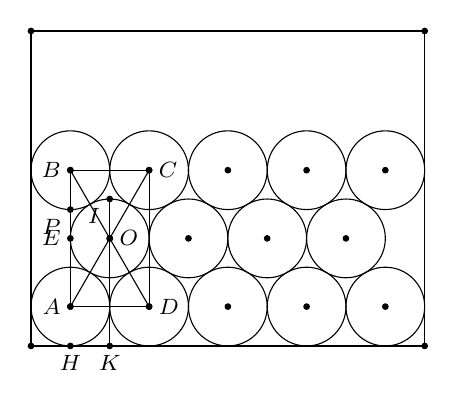
\begin{tikzpicture}[scale=1, font=\footnotesize, line join=round, line cap=round, >=stealth]
			\pgfmathsetmacro{\a}{1}
			\pgfmathsetmacro{\r}{\a/2}
			\draw(0,0)coordinate(A)rectangle+(60:{2*\a})coordinate(C);
			\draw (A|-C)coordinate(B)--(A-|C)coordinate(D)(A)--(C);
			\path (barycentric cs:A=1/2,C=1/2)coordinate(O)
			(barycentric cs:A=1/2,B=1/2)coordinate(E)
			([shift={(-90:\r)}]B)coordinate(P)
			([shift={(-135:{\r*sqrt(2)})}]A)coordinate(a)
			([shift={(-45:{\r*sqrt(2)})}]A)coordinate(K)
			([shift={(-90:\r)}]A)coordinate(H)
			([shift={(90:\r)}]O)coordinate(I);
			\draw(I)--(K)
			(a)--++(0:10*\r)coordinate(b)--++(90:8*\r)coordinate(c)--(a|-c)coordinate(d)--cycle;
			\foreach \p in {a,b,c,d} \draw[fill=black](\p)circle(1.0pt);
			\foreach \i in {0,...,4}{
				\draw(A)+(2*\i*\r,0)circle(\r);
				\draw(A)+(2*\i*\r,0)[fill=black]circle(1pt);
				\draw(B)+(2*\i*\r,0)circle(\r);
				\draw(B)+(2*\i*\r,0)[fill=black]circle(1pt);
			}
			\foreach \i in {0,...,3}{
				\draw(O)+(2*\i*\r,0)circle(\r);
				\draw(O)+(2*\i*\r,0)[fill=black]circle(1pt);
			}
			\foreach \p/\pos in{
				A/left,B/left,
				C/right,I/below left,
				O/right,E/left,K/below,
				H/below,P/below left,
				D/right}\draw[fill=black](\p)circle(1.0pt)node[\pos]{$\p$};
			\end{tikzpicture}
		\end{center}
		Nếu xếp toàn bộ các hàng $5$ viên thì chỉ xếp được $30$ hàng nên số viên phẩn xếp được là $5\cdot 30=150$ (viên).\\
		Nếu xếp toàn bộ các hàng $4$ viên thì cũng chỉ xếp được $30$ hàng nên số viên phẩn xếp được là $4\cdot 30=120$ (viên).\\
		Do đó để xếp được nhiều nhất ta xếp tối đa các viên phấn vào một cạnh chiều rộng của hộp thì được $5$ viên, hàng tiếp theo ta xếp xen kẽ $4$ viên, rồi lại xen kẽ hàng tiếp theo $5$ viên như trên hình vẽ (xét góc nhìn từ phía trên hộp xuống).\\
		Khi đó ta có $AB=\sqrt{BD^2-AD^2}=\sqrt{2^2-1}=\sqrt{3}$ nên $HP=AB+AH-BP=\sqrt{3}+\dfrac{1}{2}-\dfrac{1}{2}=\sqrt{3}$.\\
		Ta qui ước xếp hàng $5$ viên và hàng $4$ viên liên tiếp từ đầu là một cặp.\\
		Do đó ta xếp $16$ cặp trước thì diện tích khoảng trống còn lại sau khi xếp $16$ cặp này là $30-16\sqrt{3}\approx 2{,}287$.\\
		Vì $KI=OK+OI=HE+OI=\sqrt{3}+\dfrac{1}{2}\approx 2{,}23<2{,}287$ nên khoảng trống còn lại sau khi xếp $16$ cặp vừa đủ xếp cặp $17$.\\
		Vậy số phấn nhiều nhất là $17\cdot 9=153$ (viên).}
\end{ex}
\begin{ex}%[2H2G1-5]%Câu 30.
	Cho khối trụ có hai đáy là hai hình tròn $(O;R)$ và $(O';R)$, $OO'=4R$. Trên đường tròn $(O;R)$ lấy hai điểm $A, B$ sao cho $AB=a\sqrt{3}$. Mặt phẳng $(P)$ đi qua $A$, $B$ cắt đoạn $OO'$ và tạo với đáy một góc $60^{\circ}$, $(P)$ cắt khối trụ theo thiết diện là một phần của elip. Diện tích thiết diện đó bằng
	\choice
	{\True $\left(\dfrac{4\pi}{3}+\dfrac{\sqrt{3}}{2}\right)R^2$}
	{$\left(\dfrac{2\pi}{3}-\dfrac{\sqrt{3}}{4}\right)R^2$}
	{$\left(\dfrac{2\pi}{3}+\dfrac{\sqrt{3}}{4}\right)R^2$}
	{$\left(\dfrac{4\pi}{3}-\dfrac{\sqrt{3}}{2}\right)R^2$}
	\loigiai{
		\textbf{Cách 1:} Gọi $I$, $H$, $K$, $E$ là các điểm như hình vẽ.
		\immini{
			* Ta có: $\widehat{IHO}=60^{\circ}$.\\
			$OH^2=OB^2-BH^2=R^2-\dfrac{3R^2}{4}=\dfrac{R^2}{4}\Rightarrow OH=\dfrac{R}{2}$.\\
			$\Rightarrow OI=OH\cdot\tan 60^{\circ}=\dfrac{R\sqrt{3}}{2}$, $IH=\dfrac{OH}{\cos 60^{\circ}}=R$.\\
			$\triangle IOH\sim\triangle EKH$ nên ta có $\dfrac{IE}{IH}=\dfrac{OK}{OH}=2\Rightarrow IE=2R$.\\
			* Chọn hệ trục tọa độ $Ixy$ như hình vẽ, ta có elip $(E)$ có bán trục lớn là $a=IE=2R$ và $(E)$ đi qua $A\left(-R;\dfrac{R\sqrt{3}}{2}\right)$.\\
			$\Rightarrow (E)$ có phương trình là $(E)\colon\dfrac{x^2}{4R^2}+\dfrac{y^2}{R^2}=1$.\\
		}{
			\begin{tikzpicture}[scale=1, font=\footnotesize, line join=round, line cap=round, >=stealth]
			\tkzDefPoints{0/0/O,-2.08/0/D,2.08/3/C',-2.08/3/D'}
			\tkzDefPoints{2.08/1.75/p,2.08/1.8/E,2.08/0/K}
			\coordinate (A) at ($(O)+(125:2.08cm and 0.83 cm)$);
			\coordinate (B) at ($(O)+(-108:2.08cm and 0.83 cm)$);
			\coordinate (O') at ($(O)+(0,3)$);
			\tkzInterLL(O,K)(A,B)\tkzGetPoint{H}
			\tkzInterLL(H,E)(O,O')\tkzGetPoint{I}
			\tkzDefPointBy[rotation=center I angle -90](H)\tkzGetPoint{J}
			\draw (C') arc (0:360:2.08 and 0.83);
			\draw[dashed,rotate=35] (p) arc (-17:103:2.82 and 0.8);
			\draw[rotate=35] (p) arc (-17:-110.5:2.82 and 0.8);
			\draw (K) arc (0:-180:2.08 and 0.83);
			\draw[dashed] (K) arc (0:180:2.08 and 0.83);
			\coordinate (x) at ($(H)!1.3!(E)$);
			\draw[->] (H)--(x) node [below right]{$x$};
			\coordinate (y) at ($(I)!1.4!(J)$);
			\draw[->] (J)--(y) node [left]{$y$};
			\tkzDrawLines[add=0.8cm and 0cm](I,J)
			\draw (K)--(C') (D)--(D') (O')--(C');
			\draw[dashed] (A)--(B) (H)--(K) (O)--(O');
			\tkzMarkRightAngle[size=0.2](E,I,y)
			\tkzDrawPoints[fill=black,size=3](A,B,E,K,O,D,C',D',H,I)
			\tkzLabelPoints[above left](A)
			\tkzLabelPoints[below](B)
			\tkzLabelPoints[below left](H,O)
			\tkzLabelPoints[left](O',I)
			\tkzLabelPoints[below right](K,E)
			\end{tikzpicture}
		}
		\noindent
		* Diện tích của thiết diện là $S=2\displaystyle\int\limits_{-R}^{2R} R\sqrt{1-\dfrac{x^2}{4R^2}}\mathrm{\,d}x=2R\displaystyle\int\limits_{-R}^{2R}\sqrt{1-\dfrac{x^2}{4R^2}}\mathrm{\,d}x$.\\
		* Xét tích phân: $I=\displaystyle\int\limits_{-R}^{2R}\sqrt{1-\dfrac{x^2}{4R^2}}\mathrm{\,d}x$, đặt $x=2R\cdot\sin t; t\in\left[-\dfrac{\pi}{2};\dfrac{\pi}{2}\right]$ ta được
		$$I=\dfrac{R}{2}\displaystyle\int\limits_{-\tfrac{\pi}{6}}^{\tfrac{\pi}{2}}(1+\cos 2t)\mathrm{\,d}t=\dfrac{R}{2}\left(t+\dfrac{\sin 2t}{2}\right)\bigg|_{-\tfrac{\pi}{6}}^{\tfrac{\pi}{2}}=\left(\dfrac{2\pi}{3}+\dfrac{\sqrt{3}}{8}\right)R\Rightarrow S=\left(\dfrac{4\pi}{3}+\dfrac{\sqrt{3}}{4}\right)R^2.$$
		\immini{
			\textbf{Cách 2:}\\
			Ta có $\cos\widehat{AOB}=\dfrac{OA^2+OB^2-AB^2}{2\cdot OA\cdot OB}=-\dfrac{1}{2}\Rightarrow\widehat{AOB}=120^{\circ}\Rightarrow OH=\dfrac{R}{2}$.\\
			Chọn hệ trục tọa độ $Oxy$ như hình vẽ.\\
			$\Rightarrow$ Phương trình đường tròn đáy là $x^2+y^2=R^2\Leftrightarrow y=\pm\sqrt{R^2-x^2}$.\\
			Hình chiếu của phần elip xuống đáy là miền sọc như hình vẽ.\\
			Ta có $S=2\displaystyle\int\limits_{-\tfrac{R}{2}}^R\sqrt{R^2-x^2}\mathrm{\,d}x$.\\
			 Đặt $x=R\cdot\sin t\Rightarrow S=\left(\dfrac{2\pi}{3}+\dfrac{\sqrt{3}}{4}\right)R^2$.\\
			Gọi diện tích phần elip cần tính là $S'$.\\
		}{
			\begin{tikzpicture}[scale=0.8, font=\footnotesize, line join=round, line cap=round, >=stealth]
			\draw[pattern=north east lines, pattern color=gray!40, opacity=1] (0,0) circle(2cm);
			\coordinate (A) at ($(0,0)+(120:2cm)$);
			\coordinate (B) at ($(0,0)+(-120:2cm)$);
			\draw (A)--(B);
			\draw[fill=white] (A) arc (120:240:2cm and 2cm);
			\draw[->] (-2.5,0)--(3,0) node [below]{$y$};
			\draw[->] (0,-2.5)--(0,3) node [left]{$x$};
			\node at (0,0) [below left]{$O$};
			\tkzDrawPoints[fill=black,size=4](A,B)
			\tkzLabelPoints[above](A)
			\tkzLabelPoints[below](B)
			\end{tikzpicture}
		}
	Theo công thức hình chiếu, ta có $S'=\dfrac{S}{\cos 60^{\circ}}=2 S=\left(\dfrac{4\pi}{3}+\dfrac{\sqrt{3}}{2}\right)R^2$.
	}
\end{ex}
%%%%%%
%Nguyễn Tâm Phuc
\begin{ex}%[Nguyen Tam Phuc]%[2H2B1-1]%Câu 20.
	\immini{Tam giác vuông cân $ABC$ có $AB=AC=a\sqrt{2}$ và hình chữ nhật $MNPQ$ với $MQ=2MN$ được xếp chồng lên nhau sao cho $M$, $N$ lần lượt là trung điểm của $AB$, $AC$ (như hình vẽ). Tính thể tích $V$ của vật thể tròn xoay khi quay mô hình trên quanh trục $AI$, với $I$ là trung điểm $PQ$. 	
		\choice
		{$V=\dfrac{11\pi a^3}{6}$}
		{$V=\dfrac{5\pi a^3}{6}$}
		{$V=\dfrac{11\pi a^3}{8}$}
		{\True $V=\dfrac{17\pi a^3}{24}$}
	}{
		\begin{tikzpicture}[line cap=round,line join=round,>=stealth,x=1.0cm,y=1.0cm,scale=1]
		\tkzDefPoints{0/5/A,-2/3/B,2/3/C,0/3/D,0/4/E,0/0/I,0/3/F,-1/4/M,1/4/N,1/0/P,-1/0/Q}
		\tkzDrawPoints[fill=black,size=4pt](A,B,C,I,M,N,P,Q)
		\tkzLabelPoint[above](A){$A$};
		\tkzLabelPoints[below](Q,I,P);
		\tkzLabelPoints[left](M,B);
		\tkzLabelPoints[right](N,C);
		\tkzDrawSegments(A,B B,C C,A M,N M,Q Q,P P,N A,I);
		\tkzMarkRightAngles[size=.2](B,A,C);
		\end{tikzpicture} 
	}
	\loigiai{
		\immini{Ta có $BC=\sqrt{AB^2+AC^2}=2a\Rightarrow MN=a$, $MQ=2a$.\\
			Gọi $E$, $F$ lần lượt là trung điểm $MN$ và $BC$.\\ 
			Ta có $AF=a$, $EF=\dfrac{a}{2}\Rightarrow IF=\dfrac{3}{2}a$.\\
			Vậy, thể tích cần tìm
			\begin{eqnarray*}
				&V&=\dfrac{1}{3}\pi\cdot AF\cdot FB^2+\pi\cdot IF\cdot IQ^2\\
				&&=\dfrac{1}{3}\pi\cdot a\cdot a^2+\pi\cdot\dfrac{3}{2}a\cdot\left(\dfrac{a}{2}\right)^2\\
				&&=\dfrac{17}{24}\pi a^3.
			\end{eqnarray*}		
		}{
			\begin{tikzpicture}[line cap=round,line join=round,>=stealth,x=1.0cm,y=1.0cm,scale=1]
			\tkzDefPoints{0/5/A,-2/3/B,2/3/C,0/3/D,0/4/E,0/0/I,0/3/F,-1/4/M,1/4/N,1/0/P,-1/0/Q}
			\tkzDrawPoints[fill=black,size=4pt](A,B,C,I,M,N,P,Q,E,F)
			\tkzLabelPoint[above](A){$A$};
			\tkzLabelPoints[below](Q,I,P);
			\tkzLabelPoints[left](M,B);
			\tkzLabelPoints[right](N,C);
			\tkzLabelPoints[above right](E,F)
			\tkzDrawSegments(A,B B,C C,A M,N M,Q Q,P P,N A,I);
			\tkzMarkRightAngles[size=.2](B,A,C);
			\end{tikzpicture} 
		}
	}
\end{ex}
\begin{ex}%[Nguyen Tam Phuc]%[2H2B1-1]%Câu 21.
	Cho tứ diện đều $ABCD$ có cạnh bằng $a$. Hình nón $(N)$ có đỉnh $A$ và đường tròn đáy là đường tròn ngoại tiếp tam giác $BCD$. Tính thể tích $V$ của khối nón $(N)$. 
	\choice
	{$V=\dfrac{\pi\sqrt{3}a^3}{27}$}
	{$V=\dfrac{\sqrt{6}a^3}{27}$}
	{$V=\dfrac{\pi\sqrt{6}a^3}{9}$}
	{\True $V=\dfrac{\pi\sqrt{6}a^3}{27}$}
	\loigiai{
		\immini{Gọi là $O$ tâm của tam giác đều $BCD$.\\
			Ta có $AO=h$, $OC=r$ suy ra $r=\dfrac{2}{3}\dfrac{a\sqrt{3}}{2}=\dfrac{a\sqrt{3}}{3}$.\\
			Khi đó $h^2=a^2-r^2=a^2-\left(\dfrac{a\sqrt{3}}{3}\right)^2=\dfrac{2a^2}{3}\Rightarrow h=\dfrac{a\sqrt{2}}{\sqrt{3}}$.\\
			Vậy thể tích khối nón $V=\dfrac{1}{3}\pi r^2h=\dfrac{1}{3}\pi\cdot \dfrac{a^2}{3}\cdot \dfrac{a\sqrt{2}}{\sqrt{3}}=\dfrac{\pi\sqrt{6}a^3}{27}$.
		}{
			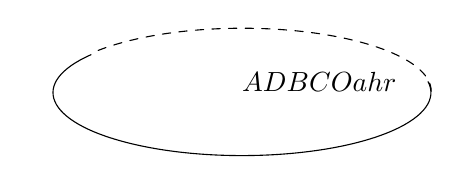
\begin{tikzpicture}[line cap=round,line join=round,>=stealth,x=1.0cm,y=1.0cm,scale=0.8]
			\tkzDefPoints{0/5/A, -2.4/0.58/B, -0.52/-0.98/C,2.87/0.31/D,0/0/O}
			\draw[dashed] (3,0) arc (0:140: 3 cm and 1 cm);
			\draw (-2.4,0.58) arc (-217:10: 3 cm and 1 cm);
			\tkzDrawPoints[fill=black,size=4pt](A,B,C,D,O)
			\tkzDrawSegments(A,B A,C A,D B,C C,D);
			\tkzDrawSegments[dashed](A,O C,O B,D);
			\tkzLabelPoint[above](A){$A$};
			\tkzLabelPoint[right](D){$D$};
			\tkzLabelPoint[above left](B){$B$};
			\tkzLabelPoint[below](C){$C$};
			\tkzLabelPoint[right](O){$O$};
			\tkzLabelPoint[left](-1.22,2.76){$a$};
			\tkzLabelPoint[right](0.12,2.16){$h$};
			\tkzLabelPoint[right](-0.24,-0.5){$r$};
			\end{tikzpicture} 
		}
	}
\end{ex}
\begin{ex}%[Nguyen Tam Phuc]%[2H2B1-2]%Câu 22.
	Cho hình chóp tam giác đều $S.ABC$ có cạnh đáy bằng $a$, góc giữa mặt bên và đáy bằng $60^{\circ}$. Diện tích xung quanh của hình nón đỉnh $S$, có đáy là hình tròn ngoại tiếp tam giác $ABC$ bằng
	\choice
	{$\dfrac{\pi a^2\sqrt{10}}{8}$}
	{$\dfrac{\pi a^2\sqrt{3}}{3}$}
	{$\dfrac{\pi a^2\sqrt{7}}{4}$}
	{\True $\dfrac{\pi a^2\sqrt{7}}{6}$}
	\loigiai{
		\immini{Gọi $I$ là tâm đường tròn $(ABC)$, suy  ra $ IA=r=\dfrac{a\sqrt{3}}{3}$.\\
			Gọi $M$ là trung điểm của $AB$, suy ra $ AB\perp(SMC)$ \\
			Suy ra góc giữa mặt bên và mặt đáy là góc $\widehat{SMC}=60^{\circ} $\\
			$\Rightarrow SM=2IM=\dfrac{2a\sqrt{3}}{6} =\dfrac{a\sqrt{3}}{3}$\\
			$\Rightarrow SA=\sqrt{SM^2+MA^2} =\sqrt{\dfrac{a^2}{3}+\dfrac{a^2}{4}} =\dfrac{a\sqrt{21}}{6}$.\\
			Diện tích xung quanh hình nón $$S_{\text{xq}}=\pi rl =\pi\cdot\dfrac{a\sqrt{3}}{3}\cdot\dfrac{a\sqrt{21}}{6} =\dfrac{\pi a^2\sqrt{7}}{6}.$$
		}{
			\begin{tikzpicture}[line cap=round,line join=round,>=stealth,x=1.0cm,y=1.0cm,scale=0.8]
			\tkzDefPoints{0/5/S,2.59/0.31/A,-0.37/-0.6/B,-2.23/0.4/C,0/0.05/I}
			\tkzDefMidPoint(A,B) \tkzGetPoint{M};
			\draw[dashed,thin] (3,0) arc (0:180:3 cm and .6 cm);
			\draw(-3,0) arc (-180:0:3 cm and .6 cm);
			\tkzDrawSegments(S,B);
			\draw(0,5) -- (-3,0);
			\draw(0,5) -- (3,0);
			\tkzDrawSegments[dashed](S,C S,I S,A S,M C,M B,C A,B);
			\tkzLabelPoint[above](S){$S$};
			\tkzLabelPoints[below](C,B,A);
			\tkzLabelPoint[below](I){$I$};
			\tkzLabelPoint[above right](M){$M$};
			\tkzDrawPoints[fill=black,size=4pt](S,A,B,C,I,M)
			\end{tikzpicture} 
		}
	}
\end{ex}
\begin{ex}%[Nguyen Tam Phuc]%[2H2G2-5]%Câu 23.
	Giá trị lớn nhất của thể tích khối nón nội tiếp trong khối cầu có bán kính $R$ là
	\choice
	{$\dfrac{1}{3}\pi R^3$}
	{$\dfrac{4}{3}\pi R^3$}
	{$\dfrac{4\sqrt{2}}{9}\pi R^3$}
	{\True $\dfrac{32}{81}\pi R^3$}
	\loigiai{
		\immini{Rõ ràng trong hai khối nón cùng bán kính đáy nội tiếp trong một khối cầu thì khối nón có chiều cao lớn hơn thì thể tích lớn hơn, nên ta chỉ xét khối nón có chiều cao lớn hơn trong hai khối nón đó.\\
			Giả sử rằng khối nón có đáy là hình tròn $(C)$ bán kính $r$. \\
			Gọi $x$ với $0\leq x <R$ là khoảng cách giữa tâm khối cầu đến đáy khối nón.\\
			Khi đó chiều cao lớn nhất của khối nón nội tiếp khối cầu với đáy là hình tròn $(C)$ sẽ là $h=R+x$. \\
			Khi đó bán kính đáy nón là $r=\sqrt{R^2-x^2}$.\\
			Vậy thể tích khối nón là
			\begin{eqnarray*}
				&V&=\dfrac{1}{3}\pi r^2h=\dfrac{1}{3}\pi(R+x)\left(R^2-x^2\right)\\
				&&=\dfrac{1}{3}\pi(R+x)(R+x)(R-x)\\
				&&=\dfrac{1}{6}\pi(R+x)(R+x)(2R-2x).
			\end{eqnarray*}	
		}{
			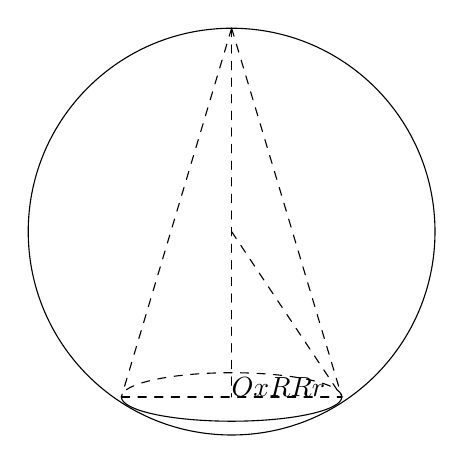
\begin{tikzpicture}[line cap=round,line join=round,>=stealth,x=1.0cm,y=1.0cm,scale=.7]
			\draw (0,3) ellipse (3.69 cm and 3.69 cm);
			\draw[dashed,thin] (2,0) arc (0:180:2 cm and 0.44 cm);
			\draw(-2,0) arc (-180:0:2 cm and 0.44 cm);
			\draw[dashed](-2,0) -- (2,0);
			\draw[dashed](0,6.69) -- (0,0);
			\draw[dashed](0,6.69) -- (-2,0);
			\draw[dashed](0,6.69) -- (2,0);
			\draw[dashed](0,3) -- (2,0);
			\tkzDrawPoint[fill=black,size=4pt](0,6.69);
			\tkzDrawPoint[fill=black,size=4pt](0,0);
			\tkzDrawPoint[fill=black,size=4pt](0,3);
			\tkzLabelPoint[left](0,3){$O$};
			\tkzLabelPoint[left](0,1.5){$x$};
			\tkzLabelPoint[left](0,4){$R$};
			\tkzLabelPoint[below](0.8,1.54){$R$};
			\tkzLabelPoint[below](1,0){$r$};
			\end{tikzpicture} 		
		}			
		\noindent Áp dụng BĐT Cô-si ta có $V\leq\dfrac{1}{6}\pi\dfrac{\left(R+x+R+x+2R-2x\right)^3}{27}=\dfrac{32\pi R^3}{81}$.}
\end{ex}
\begin{ex}%[Nguyen Tam Phuc]%[2H2G1-5]%Câu 24.
	Gọi $r$ và $h$ lần lượt là bán kính đáy và chiều cao của một hình nón. Kí hiệu $V_1$, $V_2$ lần lượt là thể tích của hình nón và thể tích của khối cầu nội tiếp hình nón. Giá trị bé nhất của tỉ số $\dfrac{V_1}{V_2}$ là
	\choice
	{$\dfrac{5}{4}$}
	{$\dfrac{4}{3}$}
	{$3$}
	{\True $2$}
	\loigiai{
		\immini{Ta có thể tích khối nón là $V_1=\dfrac{1}{3}\pi r^2h$.\\
			Xét mặt cắt qua tâm $SAB,$ kẻ tia phân giác của góc $\widehat{SBO}$, cắt $SO$ tại $I$.\\
			Ta có $\dfrac{IO}{IS}=\dfrac{OB}{SB}=\dfrac{r}{\sqrt{r^2+h^2}}\Rightarrow IS=IO\cdot\dfrac{\sqrt{r^2+h^2}}{r}$.\\
			Mặt khác $IO+IS=h$.\\
			Do đó ta có bán kính của mặt cầu nội tiếp hình chóp là $$R=IO=\dfrac{rh}{r+\sqrt{h^2+r^2}}.$$
			Thể tích khối cầu là $V_2=\dfrac{4}{3}\pi R^3=\dfrac{4}{3}\pi\dfrac{r^3h^3}{\left(r+\sqrt{h^2+r^2}\right)^3}$.
		}{
			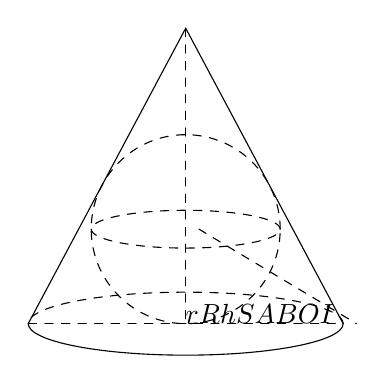
\begin{tikzpicture}[line cap=round,line join=round,>=stealth,x=1.0cm,y=1.0cm,scale=0.8]
			\draw[dashed,thin] (1.5,1.5) arc (0:360:1.5 cm and 1.5 cm);
			\draw[dashed,thin] (2.5,0) arc (0:180:2.5 cm and 0.5 cm);
			\draw (-2.5,0) arc (-180:0:2.5 cm and 0.5 cm);
			\draw[dashed,thin] (1.5,1.5) arc (0:180:1.5 cm and 0.3 cm);
			\draw[dashed,thin] (-1.5,1.5) arc (-180:0:1.5 cm and 0.3 cm);
			\draw(-2.5,0) -- (0,4.69);
			\draw(2.5,0) -- (0,4.69);
			\draw[dashed](-2.5,0) -- (2.5,0);
			\draw[dashed](0,4.69) -- (0,0);
			\tkzLabelPoint[below](1.2,0){$r$};
			\draw[dashed](0,1.5) -- (2.5,0);
			\tkzLabelPoint[above](0.82,0.4){$R$};
			\tkzLabelPoint[left](0,2.2){$h$};
			\tkzLabelPoint[above](0,4.69){$S$};
			\tkzLabelPoint[left](-2.5,0){$A$};
			\tkzLabelPoint[right](2.5,0){$B$};
			\tkzLabelPoint[below](0,0){$O$};
			\tkzLabelPoint[left](0,1.5){$I$};
			\tkzDrawPoint[fill=black,size=4pt](0,4.69);
			\tkzDrawPoint[fill=black,size=4pt](-2.5,0);
			\tkzDrawPoint[fill=black,size=4pt](2.5,0);
			\tkzDrawPoint[fill=black,size=4pt](0,0);
			\tkzDrawPoint[fill=black,size=4pt](0,1.5);
			\end{tikzpicture} 
		}
		\noindent Suy ra $\dfrac{V_1}{V_2}=\dfrac{\left(r+\sqrt{r^2+h^2}\right)^3}{4rh^2}=\dfrac{\left(1+\sqrt{1+\dfrac{h^2}{r^2}}\right)^3}{4\dfrac{h^2}{r^2}}$.\\
		Đặt $t=\sqrt{1+\dfrac{h^2}{r^2}}$ ($t\geq 1$) $\Rightarrow\dfrac{V_1}{V_2}=\dfrac{(1+t)^3}{4\left(t^2-1\right)}=\dfrac{(t+1)^2}{4(t-1)}$.\\
		Đặt $f(t)=\dfrac{(t+1)^2}{t-1}$  (điều kiện: $t\geq 1$).\\
		Khi đó $f'(t)=\dfrac{t^2-2t-3}{(t-1)^2}\Rightarrow f'(t)=0\Leftrightarrow t=3$.\\
		Bảng biến thiên
		\begin{center}
			
\begin{tikzpicture}
			\tkzTabInit[espcl=2.5,lgt=1.5]
			{$t$/0.7,$f'(t)$/0.7,$f(t)$/1.7}
			{$1$,$3$,$+\infty$}
			\tkzTabLine{,-,0,+}
			\tkzTabVar{+/$+\infty$,-/$8$,+/$+\infty$}
			\end{tikzpicture}
		\end{center}
		Từ bảng biến thiên suy ra $f(t)\geq f(3)=8,\forall t\geq 1$.\\
		Suy ra $\dfrac{V_1}{V_2}\geq 2$.
	}
\end{ex}
\begin{ex}%[Nguyen Tam Phuc]%[2H2G1-5]%Câu 25.
	Trong tất cả các hình nón nội tiếp trong hình cầu có thể tích bằng $36\pi$, tìm bán kính $r$ của hình nón có diện tích xung quanh lớn nhất. 
	\choice
	{$r=\dfrac{3}{2}$}
	{$r=\dfrac{3\sqrt{2}}{2}$}
	{\True $r=2\sqrt{2}$}
	{$r=3$}
	\loigiai{
		\immini{Gọi bán kính và thể tích của hình cầu là $R$ và $V_C$.\\
			Theo giả thiết $V_C=36\pi\Leftrightarrow\dfrac{4}{3}\pi R^3=36\pi\Leftrightarrow R=3$.\\
			Diện tích xung quanh của hình nón là\\
			$S_{\text{xq}}=\pi\cdot r\cdot SA=\pi\cdot r\cdot\sqrt{SH^2+r^2}  $ \tagEX{1}
			Khi đó $\heva{&SH=SI+IH=R+IH=3+IH\\&IH=\sqrt{IA^2-HA^2}=\sqrt{R^2-r^2}=\sqrt{9-r^2}}$ \\
			$ \Rightarrow SH=3+\sqrt{9-r^2} $ \tagEX{2}
			Từ (1) và (2) $\Rightarrow S_{\text{xq}}=\pi\cdot r\cdot\sqrt{\left(3+\sqrt{9-r^2}\right)^2+r^2}$ \\
			$ \Leftrightarrow S_{\text{xq}}=\pi\cdot\sqrt{r^2\left(3+\sqrt{9-r^2}\right)^2+r^4} $.
		}{
			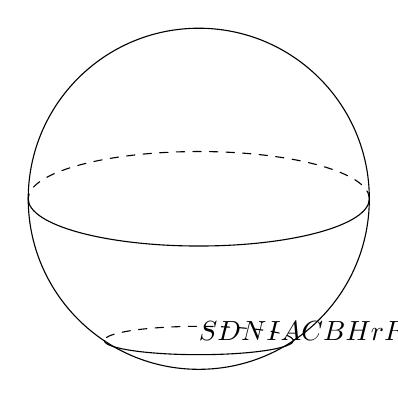
\begin{tikzpicture}[line cap=round,line join=round,>=stealth,x=1.0cm,y=1.0cm,scale=.6]
			\tkzDefPoints{-2/0/A,2/0/B,3.61/3/C,-3.61/3/D,0/0/H,0/3/I,1.09/3/M,-1.09/3/N,0/6.61/S}
			\draw (-3.61,3) arc (-180:180:3.61 cm and 3.61 cm);
			\draw[dashed,thin] (2,0) arc (0:180:2 cm and 0.3 cm);
			\draw (-2,0) arc (-180:0:2 cm and 0.3 cm);
			\draw[dashed,thin] (3.61,3) arc (0:180:3.61 cm and 1 cm);
			\draw (-3.61,3) arc (-180:0:3.61 cm and 1 cm);
			\tkzDrawSegments[dashed](S,A S,B S,H C,D A,I A,B);
			\tkzDrawPoints[fill=black,size=4pt](S,A,B,C,D,N,I,M,H)
			\tkzLabelPoint[above](S){$S$};
			\tkzLabelPoint[left](D){$D$};
			\tkzLabelPoint[above left](N){$N$};
			\tkzLabelPoint[above left](I){$I$};
			\tkzLabelPoint[left](A){$A$};
			\tkzLabelPoint[right](C){$C$};
			\tkzLabelPoint[right](B){$B$};
			\tkzLabelPoint[above left](H){$H$};
			\tkzLabelPoint[above](1,0){$r$};
			\tkzLabelPoint[above](0.5,3){$R$};
			\end{tikzpicture} 
		}
		\noindent Đặt $t=\sqrt{9-r^2}\Leftrightarrow r^2=9-t^2$. Với $0<t\leq 3$ \tagEX{3}
		\begin{eqnarray*}
			&S_{\text{xq}}&=\pi\cdot\sqrt{(9-t)^2\left(3+\sqrt{9-(9-t)^2}\right)^2+(9-t)^4}\\
			&&=\pi\cdot\sqrt{-6t^3-18t^2+54t+162}.
		\end{eqnarray*}		
		Xét hàm số 
		\begin{eqnarray*}
			&&f(t)=-6t^3-18t^2+54t+162\\
			&\Rightarrow &f'(t)=-18t^2-36t+54\\
			& \Rightarrow & f'(t)=0\Leftrightarrow \hoac{&t=-3\\&t=1.}
		\end{eqnarray*}		
		Bảng biến thiên
		\begin{center}
			\begin{tikzpicture}
			\tkzTabInit[espcl=2.5,lgt=1.7]
			{$x$/0.7,$f'(t)$/0.7,$f(t)$/1.9}
			{$0$,$1$,$3$}
			\tkzTabLine{,+,0,-}
			\tkzTabVar{-/,+/$8\sqrt{3}$,-/}
			\end{tikzpicture}
		\end{center}			
		Vậy $\max f(t)=8\sqrt{3}$ tại $t=1\Leftrightarrow \max S_{\text{xq}}=\pi 8\sqrt{3}$ tại $t=1$.\\
		Kết hợp (3) ta được $r=2\sqrt{2}$.}
\end{ex}
\begin{ex}%[Nguyen Tam Phuc]%[2H2B1-1]%Câu 26.
	\immini{Hình bên cho ta hình ảnh của một đồng hồ cát với các kích thước kèm theo $OA=OB$. Khi đó tỉ số tổng thể tích của hai hình nón $(V_n)$ và thể tích hình trụ $(V_t)$ bằng 		
		\choice
		{$\dfrac{1}{4}$}
		{$\dfrac{2}{5}$}
		{$\dfrac{1}{2}$}
		{\True $\dfrac{1}{3}$}
	}{
		\begin{tikzpicture}[line cap=round,line join=round,>=stealth,x=1.0cm,y=1.0cm,scale=.5]
		\draw[fill=blue!25, line width = 1.2pt,draw=none] (-2,6)--(0,3)--(2,6)--(-2,6);
		\draw[fill=blue!25, line width = 1.2pt,draw=none] (-2,0)--(2,0)--(0,3)--(-2,0);
		\draw[fill=blue!25] (2,6) arc (0:360:2 cm and 0.6 cm);
		\draw[dashed,thin,fill=blue!25] (2,0) arc (0:180:2 cm and 0.6 cm);
		\draw[fill=blue!25] (-2,0) arc (-180:0:2 cm and 0.6 cm);
		\draw(-2,0) -- (-2,6);
		\draw(2,0) -- (2,6);
		\draw[dashed](2,0) -- (-2,6);
		\draw[dashed](-2,0) -- (2,6);
		\tkzDrawPoint[fill=black,size=4pt](2,0);
		\tkzDrawPoint[fill=black,size=4pt](2,6);
		\draw[dashed](0,3) -- (2,3);
		\tkzLabelPoint[right](2,0){$B$};
		\tkzLabelPoint[right](2,6){$A$};
		\tkzLabelPoint[above](1,3){$R$};
		\tkzLabelPoint[right](2,3){$O$};
		\draw[<->](3,0) -- (3,6);
		\tkzLabelPoint[right](3,3){$h$};
		\end{tikzpicture} 
	}
	\loigiai{
		Thể tích của mỗi khối nón là $V_1=\dfrac{1}{3}\cdot\dfrac{h}{2}\cdot\pi R^2=\dfrac{\pi R^2h}{6}$.\\
		Tổng thể tích của hai khối nón là $V_n=2\cdot\dfrac{\pi R^2h}{6}=\dfrac{\pi R^2h}{3}$.\\
		Thể tích của khối trụ là $V_t=\pi R^2h$.\\
		Vậy $\dfrac{V_n}{V_t}=\dfrac{1}{3}$.}
\end{ex}
\begin{ex}%[Nguyen Tam Phuc]%[2H2K1-1]%Câu 27.
	\immini{Cho một đồng hồ cát như hình bên (gồm 2 hình nón chung đỉnh ghép lại), trong đó đường sinh bất kỳ của hình nón tạo với đáy một góc $60^{\circ}$ như hình bên. Biết rằng chiều cao của đồng hồ là $30$ cm và tổng thể tích của đồng hồ là $1000\pi$ cm$^3$. Hỏi nếu cho đầy lượng cát vào phần trên thì khi chảy hết xuống dưới, khi đó tỉ lệ thể tích lượng cát chiếm chỗ và thể tích phần phía dưới là bao nhiêu?
		\choice
		{$\dfrac{1}{3\sqrt{3}}$}
		{\True $\dfrac{1}{8}$}
		{$\dfrac{1}{64}$}
		{$\dfrac{1}{27}$}
	}{
		\begin{tikzpicture}[line cap=round,line join=round,>=stealth,x=1.0cm,y=1.0cm,scale=.7]
		\draw (1,5) arc (0:360:1 cm and 0.3 cm);
		\draw[dashed,thin] (2,0) arc (0:180:2 cm and 0.5 cm);
		\draw (-2,0) arc (-180:0:2 cm and 0.5 cm);
		\draw(-2,0) -- (1,5)--(-1,5)--(2,0);
		\draw[dashed](-2,0) -- (2,0);
		\draw[dashed](0,0) -- (0,5);
		\tkzDefPoints{0/0/A,-2/0/B,0/3/C}
		\tkzMarkAngles[size =0.5,mark=|,mksize=2](A,B,C);
		\tkzLabelPoint[right](-1.5,0.52){$60^{\circ}$};
		\end{tikzpicture} 
	}
	\loigiai{
		Gọi $h,h',r,r'\left(h\geq\dfrac{30}{2}=15\right)$ lần lượt là chiều cao, bán kính của hình nón phía dưới và phía trên của đồng hồ.\\
		Ta có $r=\dfrac{h}{\tan 60^{\circ}}=\dfrac{h}{\sqrt{3}};h'=30-h;r'=\dfrac{h'}{\sqrt{3}}=\dfrac{30-h}{\sqrt{3}}$.\\
		Khi đó thể tích của đồng hồ
		\begin{eqnarray*}
			&V&=\dfrac{1}{3}\pi r^2h+\dfrac{1}{3}\pi r'h'=\dfrac{1}{3}\pi\left[\left(\dfrac{h}{\sqrt{3}}\right)^2h+\left(\dfrac{30-h}{\sqrt{3}}\right)^2(30-h)\right]\\
			&&=\dfrac{1}{3}\pi\left(\dfrac{h^3+27000-2700h+90h^2-h^3}{3}\right) \\
			&&=\dfrac{1}{9}\pi\left(90h^2-2700h+27000\right)=1000\pi \\
			&& \Rightarrow h^2-30h+200=0\Leftrightarrow\hoac{&h=20\\&h=10(<15)}\Leftrightarrow h=20\Rightarrow h'=10.
		\end{eqnarray*}		
		Do $2$ hình nón đồng dạng nên $\dfrac{V_1}{V_2}=\left(\dfrac{h'}{h}\right)^3=\dfrac{1}{8}$.}
\end{ex}
\begin{ex}%[Nguyen Tam Phuc]%[2H2B1-1]%Câu 28.
	Một đống cát hình nón cụt có chiều cao $h=60$ cm, bán kính đáy lớn $R_1=1$ m, bán kính đáy nhỏ $R_2=50$ cm. Thể tích đống cát xấp xỉ
	\choice
	{$0{,}11$ m$^3$}
	{$0{,}1$ m$^3$}
	{\True $1{,}1$ m$^3$}
	{$11$ m$^3$}
	\loigiai{
		Ta có $\heva{&B=\pi R_1^2=\pi\text{ (m}^2)\\&B'=\pi R_2^2=0,25\pi\text{ (m}^2).}$\\
		Suy ra
		\begin{eqnarray*}
			&V&=\dfrac{h}{3}\left(B+B'+\sqrt{BB'}\right)\\
			&&=\dfrac{0,6}{3}\left(\pi+0,25\pi+\sqrt{\pi\cdot 0,25\pi}\right)\approx 1{,}1 \text{ (m}^3).
		\end{eqnarray*}
	}
\end{ex}
\begin{ex}%[Nguyen Tam Phuc]%[2H2G1-5]%Câu 29.
	Trong mặt phẳng với hệ trục tọa độ $Oxy,$ cho tam giác $OAB$ vuông ở $A$ thuộc trục hoành, điểm $B$ nằm trong góc phần tư thứ nhất và $OB=2017,\widehat{AOB}=\alpha,\left(0<\alpha<\dfrac{\pi}{2}\right)$. Khi quay tam giác $OAB$ quanh trục $Ox$ ta được một khối nón tròn xoay. Thể tích của khối nón đó lớn nhất khi
	\choice
	{\True $\sin\alpha=\dfrac{\sqrt{6}}{3}$}
	{$\cos\alpha=\dfrac{\sqrt{3}}{2}$}
	{$\cos\alpha=\dfrac{1}{2}$}
	{$\sin\alpha=\dfrac{\sqrt{2}}{3}$}
	\loigiai{
		\immini{Khi xoay tam giác $OAB$ quanh trục $Ox$ tạo thành hình nón có đường cao là $OA=2017\cdot\cos\alpha$ và bán kính đáy là\break $AB=OB\cdot\sin\alpha=2017\cdot\sin\alpha$.\\
			Thể tích khối nón 
			\begin{eqnarray*}
				&V&=\dfrac{1}{3}\pi\cdot AB^2\cdot OA\\
				&& =\dfrac{1}{3}\pi\left(2017\cdot\sin\alpha\right)^2\cdot 2017\cdot\cos\alpha \\
				&& =\dfrac{1}{3}\pi \cdot 2017^3\cdot \sin^2\alpha\cdot\cos\alpha\\
				&&=\dfrac{1}{3}\pi \cdot 2017^3\cdot (1-\cos ^2 \alpha)\cdot\cos\alpha.
			\end{eqnarray*}		
			\noindent Xét hàm số $f(t)=\left(1-t^2\right)t$ với $t=\cos x;t\in(0;1)$ do $\alpha\in\left(0;\dfrac{\pi}{2}\right)$.\\
		}{
			\begin{tikzpicture}[line join=round, line cap=round,>=stealth,thick,scale=1]
			\def\xmin{-1}
			\def\xmax{5}
			\def\ymin{-3}
			\def\ymax{3}
			\tikzset{label style/.style={font=\footnotesize}}
			\draw[->] (\xmin,0)--(\xmax,0) node[below left] {$x$};
			\draw[->] (0,\ymin)--(0,\ymax) node[below left] {$y$};
			\draw (0,0) node [below left] {$O$};
			\begin{scope}
			\clip (\xmin,\ymin) rectangle (\xmax,\ymax); 
			\tkzDefPoints{0/0/O,3/2/B,3/0/A}
			\draw (3.5,0) arc (0:360:0.5 cm and 2 cm);
			\draw(O) -- (A)--(B)--(O);		
			\tkzLabelPoints[above](B);	
			\tkzLabelPoints[below right](A);		
			\tkzMarkRightAngles[size=.2](B,A,O);
			\tkzMarkAngles[size =0.5,mark=|,mksize=2](A,O,B);
			\tkzLabelPoint[right](0.5,0.2){$\alpha$};
			\draw(0,0) -- (3,-2);
			\draw(3,0) -- (3,-2);
			\tkzLabelPoint[above](1.5,1.2){$2017$};
			\end{scope}
			\end{tikzpicture}		
		}
		\noindent Ta có $f'(t)=-3t^2+1$.\\
		Ta có bảng biến thiên
		\begin{center}
			\begin{tikzpicture}
			\tkzTabInit[espcl=3,lgt=1.6]
			{$x$/1.3,$f'(t)$/0.7,$f(t)$/2}
			{$0$,$\dfrac{\sqrt{3}}{3}$,$1$}
			\tkzTabLine{,+,0,-}
			\tkzTabVar{-/,+/,-/}
			\end{tikzpicture}
		\end{center}
		Vậy thể tích khối nón lớn nhất khi $\cos\alpha=\dfrac{\sqrt{3}}{3}$ hay $\sin\alpha=\sqrt{1-\cos^2\alpha}=\dfrac{\sqrt{6}}{3}$.}
\end{ex}
\begin{ex}%[Nguyen Tam Phuc]%[2H2G1-4]%Câu 30.
	Một cơ sở sản xuất đồ gia dụng được đặt hàng làm các chiếc cốc hình nón không nắp bằng nhôm có thể tích là $V=9a^3\pi$. Để tiết kiệm sản suất và mang lại lợi nhuận cao nhất thì cơ sở sẽ sản suất những chiếc cốc hình nón có bán kính miệng cốc là $R$ sao cho diện tích nhôm cần sử dụng là ít nhất. Tính $R$?
	\choice
	{$R=\dfrac{3a}{\sqrt[3]{2}}$}
	{\True $R=\dfrac{3a}{\sqrt[6]{2}}$}
	{$R=3a$}
	{$R=\sqrt[3]{9}a$}
	\loigiai{
		\immini{
			Ta có $V=9a^3\pi=\dfrac{1}{3}\pi R^2\cdot h\Rightarrow h=\dfrac{27a^3}{R^2}$ \\
			$ \Rightarrow l=\sqrt{h^2+R^2}=\sqrt{\dfrac{(3a)^6+R^6}{R^4}} $.\\
			Do đó 
			\begin{eqnarray*}
				&S_{\text{xq}}&=\pi R\cdot l=\pi\cdot R\cdot\sqrt{\dfrac{(3a)^6+R^6}{R^4}}=\pi\sqrt{\dfrac{(3a)^6+R^6}{R^2}}\\
				&&=\pi\sqrt{\dfrac{(3a)^6}{2R^2}+\dfrac{(3a)^6}{2R^2}+R^4}\\
				&&\geq\sqrt{3}\pi\sqrt[6]{\dfrac{(3a)^6}{2R^2}\cdot\dfrac{(3a)^6}{2R^2}\cdot R^4}	=\sqrt{3}\pi\sqrt[6]{\dfrac{(3a)^{12}}{4}}=\dfrac{9\sqrt{3}\pi a^2}{\sqrt[3]{2}}.\\
			\end{eqnarray*}		
			Dấu bằng xảy ra khi $\dfrac{(3a)^6}{2R^2}=R^4\Leftrightarrow(3a)^6=2R^6\Leftrightarrow R=\dfrac{3a}{\sqrt[6]{2}}$.
		}{
			\begin{tikzpicture}[line cap=round,line join=round,>=stealth,x=1.0cm,y=1.0cm,scale=1]
			
			\tkzDefPoints{-2/4/A,2/4/B,0/4/O,0/0/S}
			\draw (B) arc (0:360:2 cm and 0.5 cm);
			\tkzDrawSegments(A,B B,S S,A);		
			\tkzDrawPoints[fill=black,size=4pt](A,B,O,S);
			\tkzLabelPoint[left](A){$A$};
			\tkzLabelPoint[right](B){$B$};
			\tkzLabelPoint[above](O){$O$};
			\draw[dashed](S) -- (O);
			\tkzLabelPoint[below](S){$S$};
			\end{tikzpicture} 
		}
	}
\end{ex}
\begin{dang}{Tính diện tích xung quanh, diện tích toàn phần và thể tích khối trụ}
\end{dang}
\subsubsection{Các ví dụ}
\begin{vd}%[Nguyen Tam Phuc]%[2H2Y1-2]%Ví dụ 1.
	Cho hình trụ có hình tròn đáy bán kính $r=a$, có hiều cao $h=a\sqrt{3}$. Tính diện tích xung quanh và diện tích toàn phần hình trụ theo $a$.
	\loigiai{
		Diện tích xung quanh $S_{\text{xq}}=2\pi rh=2\pi a^2\sqrt{3}$.\\
		Diện tích toàn phần $S_{t p}=S_{\text{xq}}+2 \cdot S_{\text{đáy}}=2 \pi r h+2 \pi r^{2}=(1+\sqrt{3}) 2 \pi a^{2}$.		}
\end{vd}
\begin{vd}%[Nguyen Tam Phuc]%[2H2Y1-2]%Ví dụ 2.
	Cho hình trụ có hình tròn đáy bán kính là $r=a$, có thiết diện qua trục là một hình vuông. Tính diện tích xung quanh và diện tích toàn phần hình trụ theo $a$.
	\loigiai{
		\immini{Gọi thiết diện qua trục là hình vuông $ABB'A'$ với $AB$, $A'B'$ lần lượt là đường kính 2 đường tròn đáy $\Rightarrow AB=A'B'=2r=2a$, do đó $h=AA'=BB'=2a$.\\
			+ Diện tích xung quanh $S_{\text{xq}}=2\pi rh=4\pi a^2$.\\
			+ Diện tích toàn phần $S_{\text{tp}}=S_{\text{xq}}+2 \cdot S_{\text {đáy}}=2 \pi r h+2 \pi r^{2}=6 \pi a^{2}$.
		}{
			\begin{tikzpicture}[line cap=round,line join=round,>=stealth,x=1.0cm,y=1.0cm,scale=1]
			\tkzDefPoints{0/0/O,0/4/O',-1.33/-0.37/A,-1.33/3.59/A',1.29/0.42/B,1.29/4.42/B'}
			\draw[dashed,thin] (2,0) arc (0:180:2 cm and 0.5 cm);
			\draw (-2,0) arc (-180:0:2 cm and 0.5 cm);
			\draw (2,4) arc (0:360:2 cm and 0.5 cm);
			\draw (A)--(A') -- (B');
			\draw[dashed](A) -- (B)--(B');
			\draw[dashed](O) -- (O');
			\tkzDrawPoints[fill=black,size=4pt](A,B,A',B',O,O');
			\tkzLabelPoints[above](A',O',B');
			\tkzLabelPoints[below](A,O);
			\tkzLabelPoint[below](B){$B$};
			\tkzMarkSegments[size=3,mark=|,
			pos=.5](A,A' B,B');
			\tkzMarkSegments[size=3,mark=||,
			pos=.5](A',O' A,O);
			\draw(-2,0) -- (-2,4);
			\draw(2,0) -- (2,4);
			\end{tikzpicture} 
		}
	}
\end{vd}

\begin{vd}%[Nguyen Tam Phuc]%[2H2K1-2]%Ví dụ 4.
	Cho một hình trụ tròn xoay và hình vuông $ABCD$ cạnh $a$ có hai đỉnh liên tiếp $A$, $B$ nằm trên đường tròn đáy thứ nhất của hình trụ, hai đỉnh còn lại nằm trên đường tròn đáy thứ hai của hình trụ. Mặt phẳng $(ABCD)$ tạo với đáy hình trụ góc $45^{\circ}$. Tính diện tích xung quanh và diện tích toàn phần hình trụ theo $a$.
	\loigiai{		
		\immini{Gọi $M$, $N$ trung điểm $AB$, $CD\Rightarrow MN$ là trục hình vuông $ABCD$ và $MN$ qua trung điểm $I$ của $OO'$.\\
			$$\left((ABCD),(ABO)\right)=(MI,MO)=\widehat{IMO}=45^{\circ}.$$
			$\triangle IOM$ vuông cân tại $O $
			\begin{eqnarray*}
				&\Rightarrow &OM=OI=\dfrac{MI}{\sqrt{2}}=\dfrac{a}{2\sqrt{2}}\\
				&\Rightarrow &h=OO'=2OI=\dfrac{a\sqrt{2}}{2}.				\end{eqnarray*}	
			$\triangle MOA$ vuông tại $M$
			\begin{eqnarray*}
				&\Rightarrow&  r=OA=\sqrt{OM^2+MA^2}\\
				&&=\sqrt{\left(\dfrac{a}{2\sqrt{2}}\right)^2+\left(\dfrac{a}{2}\right)^2}\\
				&&=\dfrac{a\sqrt{6}}{4}.\
			\end{eqnarray*}			
			+ Diện tích xung quanh $S_{\text{xq}}=2\pi rh=\dfrac{\pi\sqrt{3}}{2}a^2$.\\
			+ Diện tích toàn phần $$S_\text{tp}=S_\text{xq}+2 \cdot S_{\text{đáy}}=2 \pi r h+2 \pi r^2=\dfrac{\pi \sqrt{3}}{2} a^2+\dfrac{3 \pi}{4} a^2=\dfrac{(3+2 \sqrt{3}) \pi}{4} a^2.$$
		}{
			\begin{tikzpicture}[line cap=round,line join=round,>=stealth,x=1.0cm,y=1.0cm,scale=1]
			\tkzDefPoints{0/0/O,0/4/O',-0.97/-0.44/A,-1.48/0.35/B,0.97/4.5/C,1.52/3.66/D,-1.22/-0.01/M,1.22/4.01/N,0/2/I}
			\draw[dashed,thin] (2,0) arc (0:180:2 cm and 0.5 cm);
			\draw (-2,0) arc (-180:0:2 cm and 0.5 cm);
			\draw (2,4) arc (0:360:2 cm and 0.5 cm);
			\draw(-2,0) -- (-2,4);
			\draw(2,0) -- (2,4);
			\draw[dashed](O) -- (O');
			\draw(A) -- (D)--(C);
			\draw(-2,4) -- (2,4);
			\draw[dashed](-2,0) -- (2,0);	
			\draw[dashed](A) -- (B)--(C);
			\draw[dashed](M) -- (N);
			\tkzLabelPoints[below](A,O);
			\tkzLabelPoints[above](O',C,B);
			\tkzLabelPoints[above right](N);
			\tkzLabelPoints[below right](D);
			\tkzLabelPoints[above left,fill=white](I);
			\tkzLabelPoints[below left](M);
			\tkzDrawPoints[fill=black,size=4pt](A,B,C,D,M,N,O,O',I);	
			\draw[pattern = north east lines, line width = 1.2pt,draw=none] (A)--(B)--(C)--(D)--(A);
			\end{tikzpicture} 
		}
	}
\end{vd}
\begin{vd}%[Nguyen Tam Phuc]%[2H2K1-2]%Ví dụ 5.
	Cho hình trụ tròn xoay có hai đáy là hai hình tròn $(O,R)$ và $(O',R)$. Biết rằng tồn tại dây cung $AB$ của đường tròn $(O)$ sao cho $\Delta O'AB$ đều và mp$(O'AB)$ hợp với mặt phẳng chứa đường tròn $(O)$ một góc $60^{\circ}$. Tính diện tích xung quanh và diện tích toàn phần hình trụ theo $R$.
	\loigiai{
		\immini{Đặt độ dài cạnh tam giác đều $ABC$ là $x$.\\
			Gọi $I$ là trung điểm $AB\Rightarrow OI\perp AB, O'I\perp AB$.\\
			Lại có  $\left((O'AB),(AOB)\right)=(O'I,OI)=\widehat{O'IO}=60^{\circ}$\\
			$\Rightarrow OI=\dfrac{O'I}{2}=\dfrac{x\sqrt{3}}{4}$ và $h=OO'=O'I\dfrac{\sqrt{3}}{2}=\dfrac{3x}{4}$.\\
			$\triangle AIO$ vuông tại  $I$
			\begin{eqnarray*}
				&&\Rightarrow  OI^2+AI^2=OA^2\\
				&\Leftrightarrow & \left(\dfrac{x\sqrt{3}}{4}\right)^2+\left(\dfrac{x}{2}\right)^2=R^2\dfrac{7}{16}x^2\\
				&&\Leftrightarrow x=\dfrac{4\sqrt{7}}{7}R.
			\end{eqnarray*}
			Vậy $h=\dfrac{3x}{4}=\dfrac{3\sqrt{7}}{7}R$.\\
			+ Diện tích xung quanh $S_{\text{xq}}=2\pi rh=\dfrac{6\sqrt{7}\pi R^2}{7}$.\\
			+ Diện tích toàn phần $S_{\text{tp}}=S_{\text{xq}}+2 \cdot S_{\text {đáy}}=2 \pi r h+2 \pi r^{2}=6 \pi a^{2}$.
		}{
			\begin{tikzpicture}[line cap=round,line join=round,>=stealth,x=1.0cm,y=1.0cm,scale=1]
			\tkzDefPoints{0/0/O,0/4/O',-0.97/-0.44/A,-1.48/0.35/B,-1.22/0/I}
			\draw[dashed,thin] (2,0) arc (0:180:2 cm and 0.5 cm);
			\draw (-2,0) arc (-180:0:2 cm and 0.5 cm);
			\draw (2,4) arc (0:360:2 cm and 0.5 cm);
			\draw(-2,0) -- (-2,4);
			\draw(2,0) -- (2,4);
			\draw[dashed](O) -- (O');		
			\draw[dashed](-2,0) -- (2,0);	
			\draw(-2,4) -- (2,4);
			\draw[dashed](A) -- (B)--(O')--(A)--(O);
			\draw[dashed](I) -- (O');
			\tkzLabelPoints[below](A,O);
			\tkzLabelPoints[above](O',B);	
			\tkzDrawPoints[fill=black,size=4pt](A,B,O,O',I);	
			\draw[pattern = north east lines, line width = 1.2pt,draw=none] (A)--(B)--(O')--(A);
			\tkzLabelPoints[below left](I);
			\tkzMarkAngles[size =0.5,mark=|,mksize=2](O,I,O');
			\tkzLabelPoint[above right](I){$60^{\circ}$};
			\end{tikzpicture} 
		}
	}
\end{vd}
\subsubsection{Câu hỏi trắc nghiệm}
\begin{ex}%[Nguyen Tam Phuc]%[2H2Y1-2]%Câu 1.
	Cho hình trụ $(T)$ có chiều cao $h$, độ dài đường sinh $l$, bán kính đáy $r$. Ký hiệu $S_{\text{xq}}$ là diện tích xung quanh của $(T)$. Công thức nào sau đây là đúng?
	\choice
	{$S_{\text{xq}}=\pi rh$}
	{\True $S_{\text{xq}}=2\pi rl$}
	{$S_{\text{xq}}=2\pi r^2h$}
	{$S_{\text{xq}}=\pi rl$}
	\loigiai{
		Với hình trụ ta có $h=l\Rightarrow S_{\text{xq}}=2\pi rh=2\pi rl$.}
\end{ex}
\begin{ex}%[Nguyen Tam Phuc]%[2H2Y1-2]%Câu 2.
	Cho hình trụ $(T)$ có chiều cao $h$, độ dài đường sinh $l$, bán kính đáy $r$. Ký hiệu $S_{\text{tp}}$ là diện tích toàn phần của $(T)$. Công thức nào sau đây là đúng?
	\choice
	{$S_{\text{tp}}=\pi rl$}
	{$S_{\text{tp}}=\pi rl+2\pi r$}
	{$S_{\text{tp}}=\pi rl+\pi r^2$}
	{\True $S_{\text{tp}}=2\pi rl+2\pi r^2$}
	\loigiai{
		Ta có: $S_{\text{tp}}=S_{\text{xq}}+S_{2.d}=2\pi rh+2\left(\pi r^2\right)=2\pi rl+2\pi r^2$.}
\end{ex}
\begin{ex}%[Nguyen Tam Phuc]%[2H2Y1-1]%Câu 3.
	Cho hình trụ $(T)$ có chiều cao $h$, độ dài đường sinh $l$, bán kính đáy $r$. Ký hiệu $V_{(T)}$ là thể tích khối trụ $(T)$. Công thức nào sau đây là đúng?
	\choice
	{$V_{(T)}=\dfrac{1}{3}\pi rh$}
	{\True $V_{(T)}=\pi r^2h$}
	{$V_{(N)}=\pi rl^2$}
	{$V_{(N)}=2\pi r^2h$}
	\loigiai{
		Ta có $V_{(T)}=S_d\cdot h=\pi r^2h$.}
\end{ex}
\begin{ex}%[Nguyen Tam Phuc]%[2H2Y1-2]%Câu 4.
	Một hình trụ có bán kính đáy $r=5$ cm, chiều cao $h=7$ cm. Diện tích xung quanh của hình trụ này là
	\choice
	{$35\pi$ (cm$^2$)}
	{\True $70\pi$ (cm$^2$)}
	{$\dfrac{70}{3}\pi$ (cm$^2$)}
	{$\dfrac{35}{3}\pi$ (cm$^2$)}
	\loigiai{
		Ta có $S_{\text{xq}}=2\pi rh=2\pi\cdot 5\cdot 7=70\pi$ (cm$^2$).}
\end{ex}
\begin{ex}%[Nguyen Tam Phuc]%[2H2Y1-2]%Câu 5.
	Một hình trụ có bán kính đáy $r=a$, độ dài đường sinh $l=2a$. Diện tích toàn phần của hình trụ này là
	\choice
	{\True $6\pi a^2$}
	{$2\pi a^2$}
	{$4\pi a^2$}
	{$5\pi a^2$}
	\loigiai{
		Ta có $S_{\text{tp}}=S_{\text{xq}}+S_{2\text{đáy}}=2\pi rh+2\left(\pi r^2\right)=2\pi rl+2\pi r^2=4a^2\pi+2a^2\pi=6a^2\pi$.}
\end{ex}
\begin{ex}%[Nguyen Tam Phuc]%[2H2B1-1]%Câu 6.
	Quay hình vuông $ABCD$ cạnh $a$ xung quanh một cạnh. Thể tích của khối trụ được tạo thành là
	\choice
	{$\dfrac{1}{3}\pi a^3$}
	{$2\pi a^3$}
	{\True $\pi a^3$}
	{$3\pi a^3$}
	\loigiai{
		Khi quay hình vuông cạnh $a$ quanh $1$ cạnh ta được khối trụ có $r=h=a$.\\
		Ta có $V_{(T)}=S_d\cdot h=\pi r^2h=\pi a^3$.}
\end{ex}
\begin{ex}%[Nguyen Tam Phuc]%[2H2Y1-1]%Câu 7.
	Khối trụ có chiều cao $h=3$ cm và bán kính đáy $r=2$ cm thì có thể tích bằng
	\choice
	{\True $12\pi\text{ (cm}^3)$}
	{$4\pi\text{ (cm}^3)$}
	{$6\pi\text{ (cm}^3)$}
	{$12\pi$ (cm$^2$)}
	\loigiai{
		Thể tích của khối trụ là $V=\pi r^2h=\pi\cdot 2^2\cdot 3=12\pi$.}
\end{ex}
\begin{ex}%[Nguyen Tam Phuc]%[2H2B1-1]%Câu 8.
	Bên trong một lon sữa hình trụ có đường kính đáy bằng chiều cao và bằng $1$ dm. Thể tích thực của lon sữa đó bằng
	\choice
	{$2\pi \text{ (dm}^3)$}
	{$\dfrac{\pi}{2} \text{ (dm}^3)$}
	{\True $\dfrac{\pi}{4}\text{ (dm}^3)$}
	{$\pi\text{ (dm}^3)$}
	\loigiai{
		Thể tích thực của lon sữa hình trụ là $V=\pi r^2h=\pi\left(\dfrac{1}{2}\right)^2\cdot 1=\dfrac{\pi}{4} \text{ (dm}^3)$.}
\end{ex}
\begin{ex}%[Nguyen Tam Phuc]%[ID6]%Câu 9.
	Cho hình vuông $ABCD$ cạnh $8$ cm. Gọi $M$, $N$ lần lượt là trung điểm của $AB$ và $CD$. Quay hình vuông $ABCD$ xung quanh $MN$. Diện tích xung quanh của hình trụ tạo thành là
	\choice
	{\True $64\pi$ (cm$^2$)}
	{$32\pi$ (cm$^2$)}
	{$96\pi$ (cm$^2$)}
	{$126\pi$ (cm$^2$)}
	\loigiai{
		\immini{Quay hình vuông $ABCD$ xung quanh $MN$ ta được hình trụ như hình vẽ.\\
			Khi đó $r=\dfrac{AB}{2}=4;h=AD=8\Rightarrow S_{\text{xq}}=2\pi rh=64\pi$ (cm$^2$).
		}{
			\begin{tikzpicture}[line cap=round,line join=round,>=stealth,x=1.0cm,y=1.0cm,scale=.7]
			\draw (2,4) arc (0:360:2 cm and 0.5 cm);
			\draw[dashed,thin] (2,0) arc (0:180:2 cm and 0.5 cm);
			\draw(-2,0) arc (-180:0:2 cm and 0.5 cm);
			\draw(-2,0) -- (-2,4)--(2,4)--(2,0);
			\draw[dashed](-2,0) -- (2,0);
			\draw[dashed](0,0) -- (0,4);
			\tkzLabelPoint[left](-2,4){$A$};
			\tkzLabelPoint[right](2,4){$B$};
			\tkzLabelPoint[below](0,0){$N$};
			\tkzLabelPoint[above](0,4){$M$};
			\tkzLabelPoint[left](-2,0){$D$};
			\tkzLabelPoint[right](2,0){$C$};
			\tkzDrawPoint[fill=black,size=4pt](-2,4);
			\tkzDrawPoint[fill=black,size=4pt](2,4);
			\tkzDrawPoint[fill=black,size=4pt](0,0);
			\tkzDrawPoint[fill=black,size=4pt](0,4);
			\tkzDrawPoint[fill=black,size=4pt](-2,0);
			\tkzDrawPoint[fill=black,size=4pt](2,0);
			\end{tikzpicture} 
		}
	}
\end{ex}
\begin{ex}%[Nguyen Tam Phuc]%[2H2B1-2]%Câu 10.
	Một hình trụ $(T)$ có diện tích toàn phần là $120\pi$ (cm$^2$) và có bán kính đáy bằng $6$ cm. Chiều cao của $(T)$ là
	\choice
	{$6$ cm}
	{$5$ cm}
	{\True  $4$ cm}
	{$3$ cm}
	\loigiai{
		Ta có: $S_{\text{tp}}=S_{\text{xq}}+S_{2.d}=2\pi rh+2\left(\pi r^2\right)=12\pi h+72\pi=120\pi\Rightarrow h=4$ (cm).}
\end{ex}
\begin{ex}%[Nguyen Tam Phuc]%[2H2B1-2]%Câu 11.
	Một khối trụ $(T)$ có thể tích bằng $81\pi \text{ (cm}^3)$ và có đường sinh gấp ba lần bán kính đáy. Độ dài đường sinh của $(T)$ là
	\choice
	{$12$ cm}
	{$3$ cm}
	{$6$ cm}
	{\True $9$ cm}
	\loigiai{
		Ta có $V_{(T)}=S_d\cdot h=\pi r^2h=\pi r^2l=\pi\left(\dfrac{l}{3}\right)^2l=81\pi\Leftrightarrow l^3=729\Leftrightarrow l=9$.}
\end{ex}
\begin{ex}%[Nguyen Tam Phuc]%[2H2K1-2]%Câu 12.
	Cho hình chữ nhật $ABCD$ có $AB=a$ và góc $BDC=30^{\circ}$. Quay hình chữ nhật này xung quanh cạnh $AD$. Diện tích xung quanh của hình trụ được tạo thành là
	\choice
	{$\sqrt{3}\pi a^2$}
	{$2\sqrt{3}\pi a^2$}
	{\True $\dfrac{2}{\sqrt{3}}\pi a^2$}
	{$\pi a^2$}
	\loigiai{
		\immini{Khi quay hình chữ nhật này xung quanh cạnh $AD$ ta được hình trụ như hình vẽ. \\
			Ta có $r=AB=a;h=BC=CD\tan 30^{\circ}$.\\
			Suy ra $h=\dfrac{a}{\sqrt{3}}$.\\
			Vậy $ S_{\text{xq}}=2\pi rh=\dfrac{2\pi a^2}{\sqrt{3}}$.
		}{
			\begin{tikzpicture}[line cap=round,line join=round,>=stealth,x=1.0cm,y=1.0cm,scale=.8]
			\draw (2,4) arc (0:360:2 cm and 0.5 cm);
			\draw[dashed,thin] (2,0) arc (0:180:2 cm and 0.5 cm);
			\draw(-2,0) arc (-180:0:2 cm and 0.5 cm);
			\draw(-2,0) -- (-2,4)--(2,4)--(2,0);
			\draw[dashed](-2,0) -- (2,0);
			\draw[dashed](0,0) -- (0,4);
			\draw[dashed](0,0) -- (2,4);
			\tkzLabelPoint[above](0,4){$A$};
			\tkzLabelPoint[right](2,4){$B$};
			\tkzLabelPoint[below](0,0){$D$};
			\tkzLabelPoint[right](2,0){$C$};
			\tkzDefPoints{0/0/D,2/4/B,2/0/C}
			\tkzMarkAngles[size =0.5,mark=|,mksize=2](C,D,B);
			\tkzLabelPoint[right](0.54,0.46){$30^{\circ}$};
			\tkzDrawPoint[fill=black,size=4pt](0,0);
			\tkzDrawPoint[fill=black,size=4pt](2,0);
			\tkzDrawPoint[fill=black,size=4pt](2,4);
			\tkzDrawPoint[fill=black,size=4pt](0,4);
			\end{tikzpicture} 
		}
	}
\end{ex}
\Closesolutionfile{ans}